\documentclass[]{report}
\usepackage{systeme,mathtools}
\usepackage{graphicx}
%opening
\title{PR251 ANALYSIS}
\author{Luna Pellegri}

\begin{document}
\maketitle

\chapter{Cable offset}
\chapter{Lookuptable (LUT)}
\chapter{DATA corrections}

\section{TOF alignament}
Once the procedure of the CableLength and LUT is completed, a selection on the particle of interest must be applied to the data. Since the RF is not stable during the whole experiment a shift in the measured TOF can be seen in the data. In order to use a unique cut (pad1vstof cut) on the pad1:tof matrix a offset correction to the data must be applied\\
Retief implemented a new routine in the analyser that reads the TOF offsets from file and apply them to the different events.
The TOF offsets file must contain one column with the run number and another with the corresponding offset value. Be sure that the offset values are integers and the file ends with eof.
The file name should be add in the config.cfg file under "TOFOffsetsFile". The number of the runs in the offsets file must also be written in the config file (NrOfTOFOffsets).\\
Procedure to calculate the TOF offsets:
\begin{enumerate}
	\item Use the code get$\_$tofpeak.C to extract the TOF offsets. It extracts the TOF position of the bump marked in red in Fig. for the list of runs given and it calculates the offsets of the peak position respect to the one in the first run in the list. The calculated offsets are saved in a .dat file. Edit the file to add "eof" at the end.
	\item Put the TOFoffsets file in the Analyser folder.
	\item Modify the NrOfTOFOffsets and TOFOffsetsFile in the config.cfg file.
	\item Run the Analyser and check that the offsets have been implemented. The variable "tof" in the rootTree is now the one corrected and "toftdc1 this the uncorrected one.
\end{enumerate}

\begin{figure}
	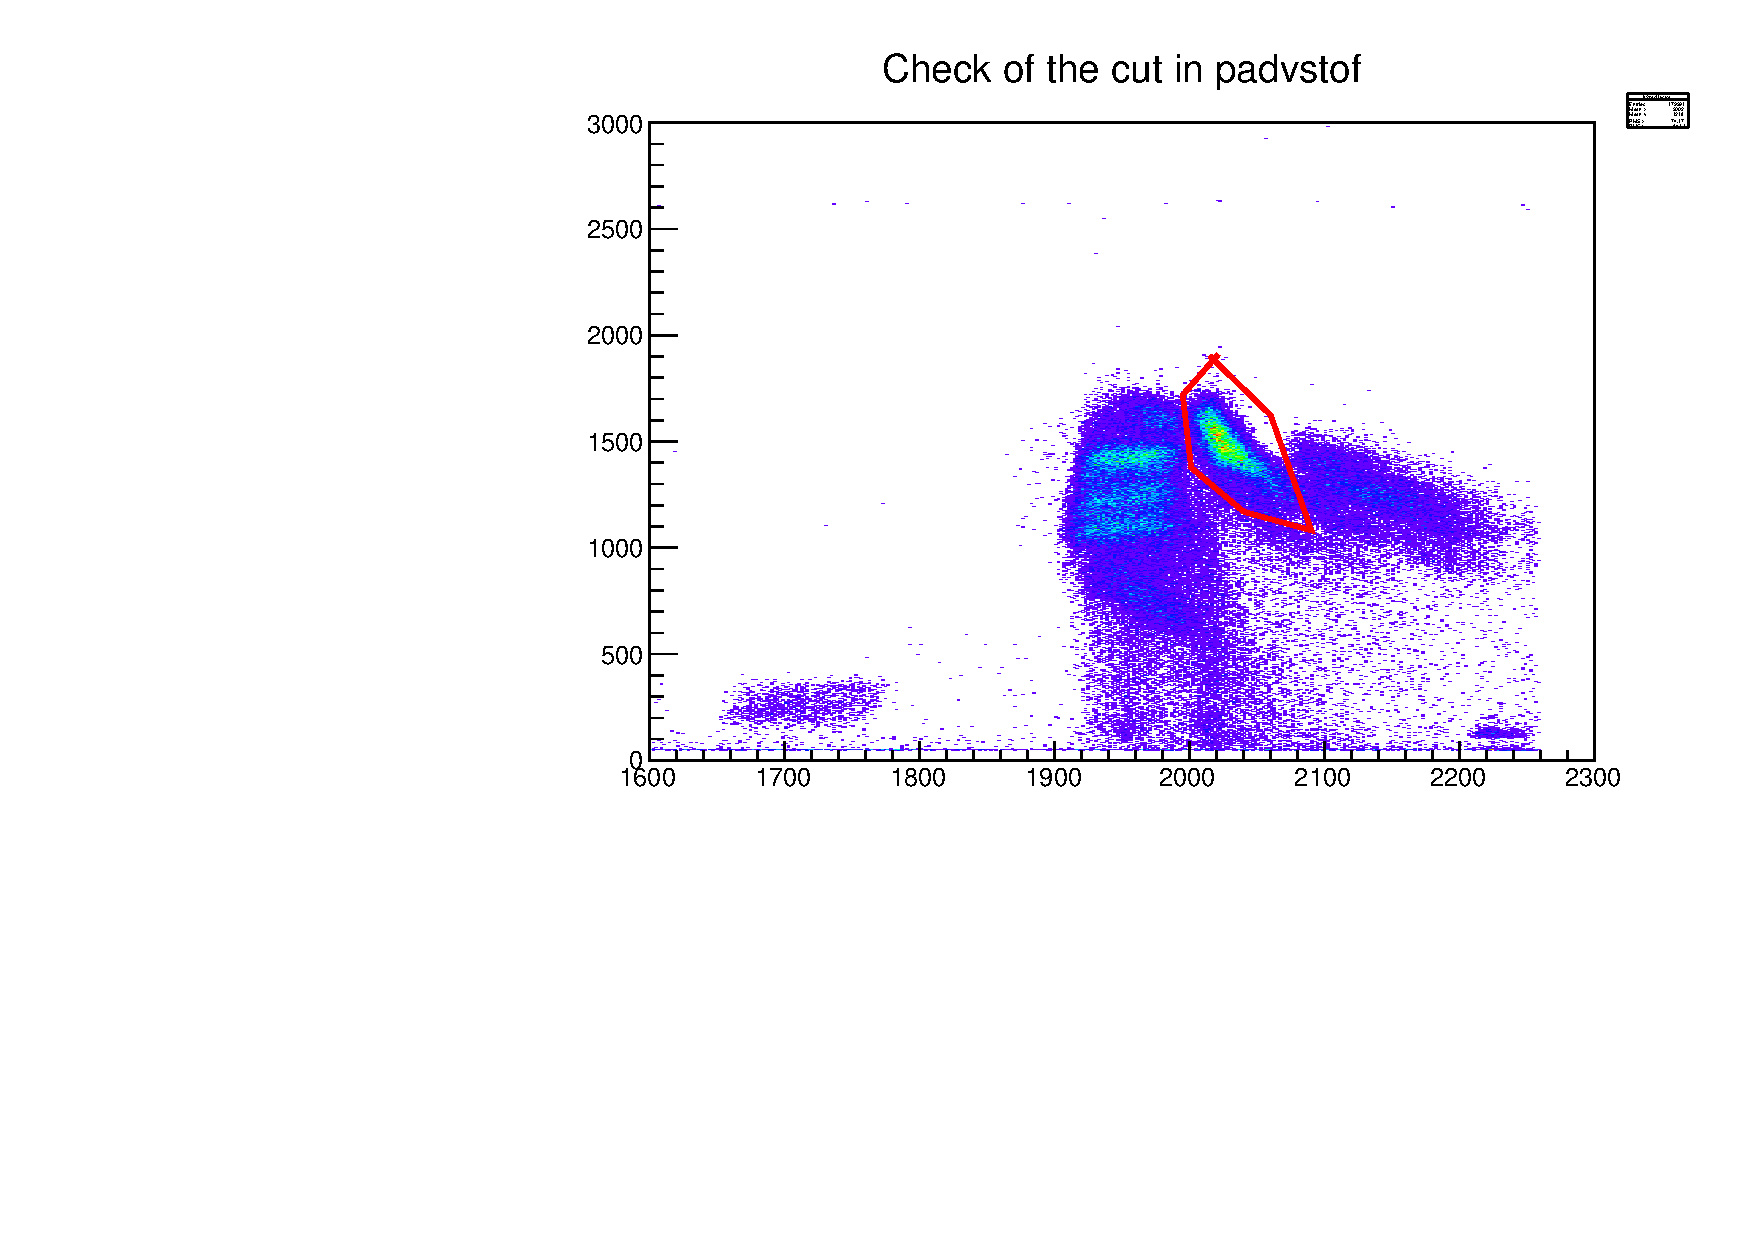
\includegraphics[width=\linewidth]{Figure/run2227-24Mg-TOFaligment-Jan18.pdf}
	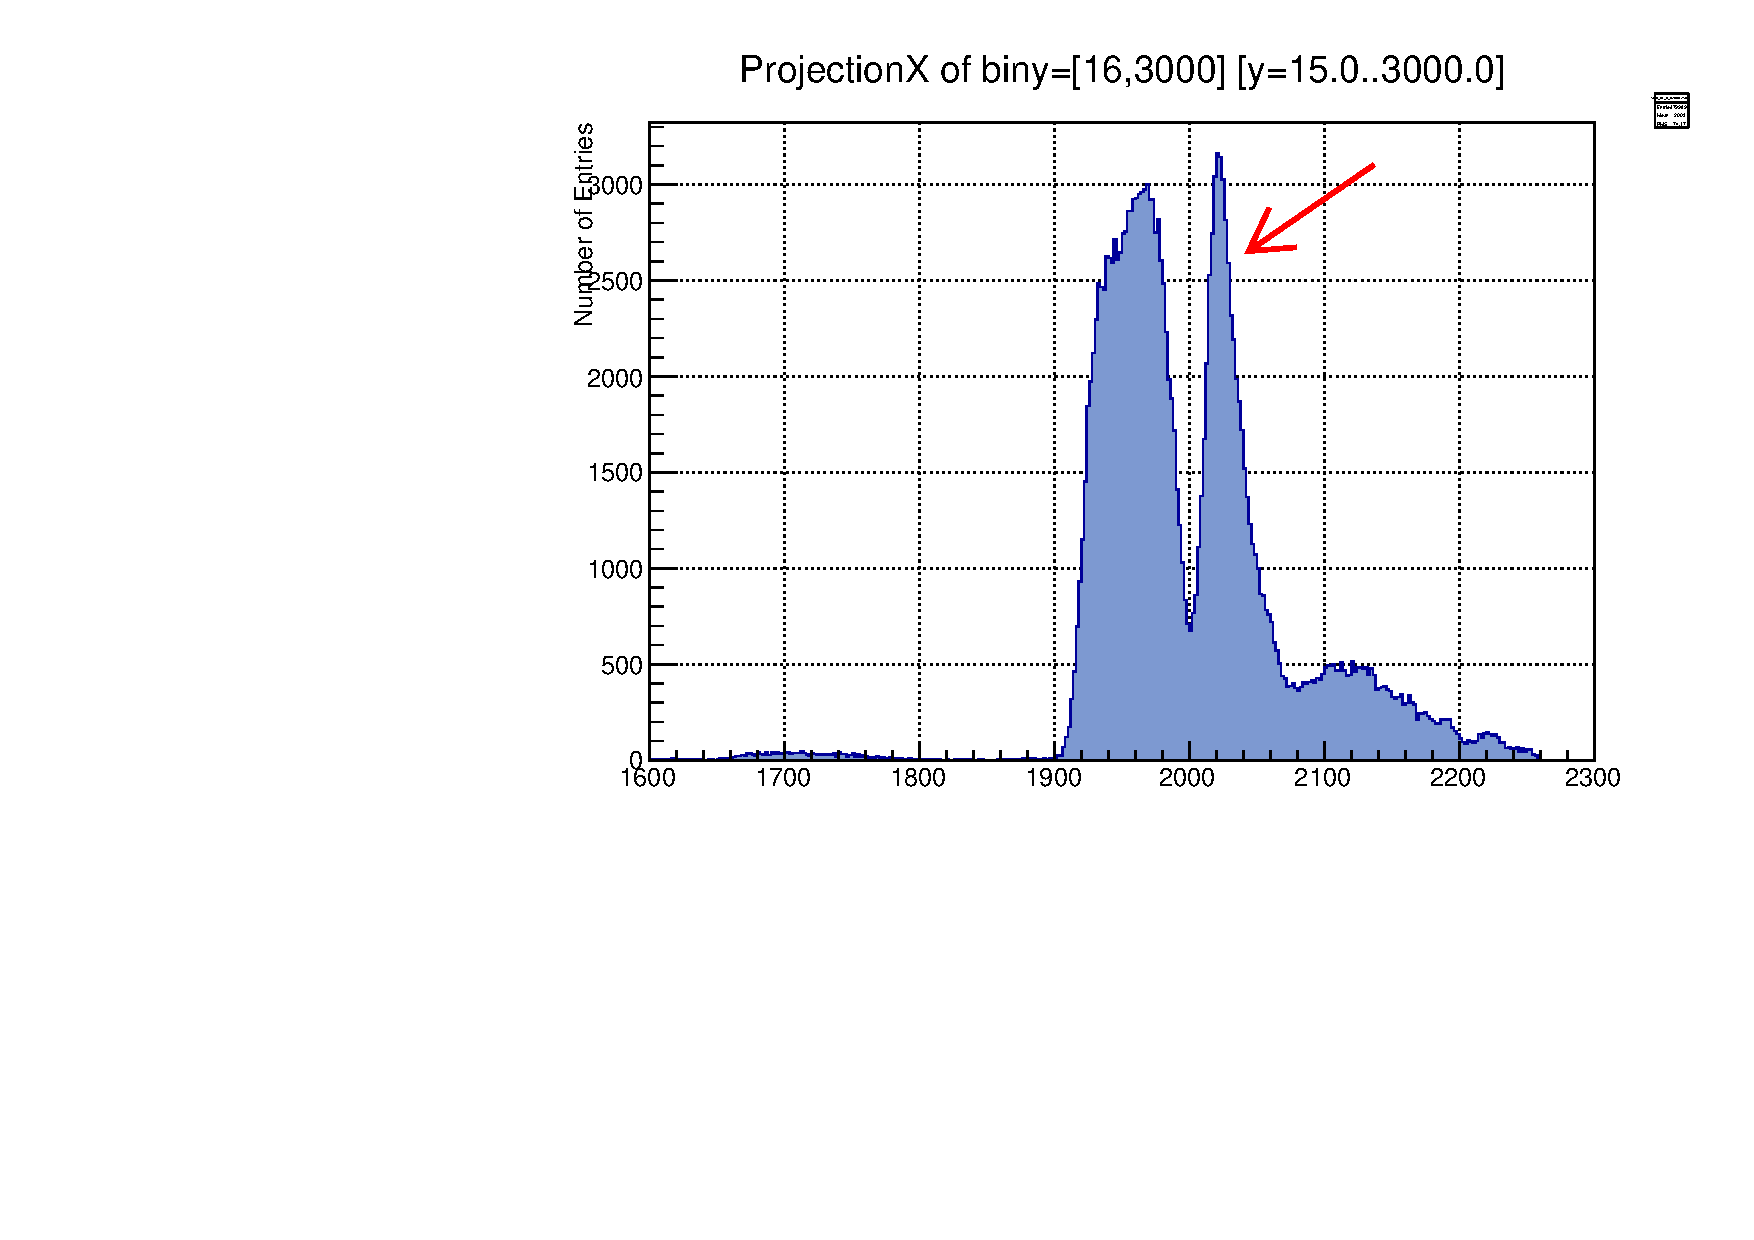
\includegraphics[width=\linewidth]{Figure/run2227-24Mg-TOFaligment-peak-Jan18.pdf}
	\caption{Tof vs X1posO for a 24Mg run. Peak used for the alignment.}
	\label{fig:tofvspad1}
\end{figure}

\section{Pad1 alignment}

Also in the case of Pad1 values an offsets correction must be applied to be able to use a unique cut on the pad1vsX1pos matrix.
The procedure is similar to the one described for the TOF
\begin{enumerate}
	\item Use the code get$\_$padpeak.C to extract the Pad1 offsets. It extracts the pad1 position of the most intense peak in the pad1vsX1 matrix for the list of runs given and it calculates the offsets of the peak position respect to the one in the first run in the list. The calculated offsets are saved in a .dat file. Edit the file to add "eof" at the end.
	\item Put the PadOffsets file in the Analyser folder.
	\item Modify the NrOfPadOffsets and PadOffsetsFile in the config.cfg file.
	\item Run the Analyser and check that the offsets have been implemented. The variable "pad1" in the rootTree is now the one corrected and "pad1raw" is the uncorrected one.
\end{enumerate}

Once these corrections have been implemented in the data, the gate to select the particle of interest (pad1vstof) and the one to select the good events from the background (pad1vsX1) can be created (see Fig. \ref{fig:pad1vstof},\ref{fig:pad1vsX1}).\\


\begin{figure}
	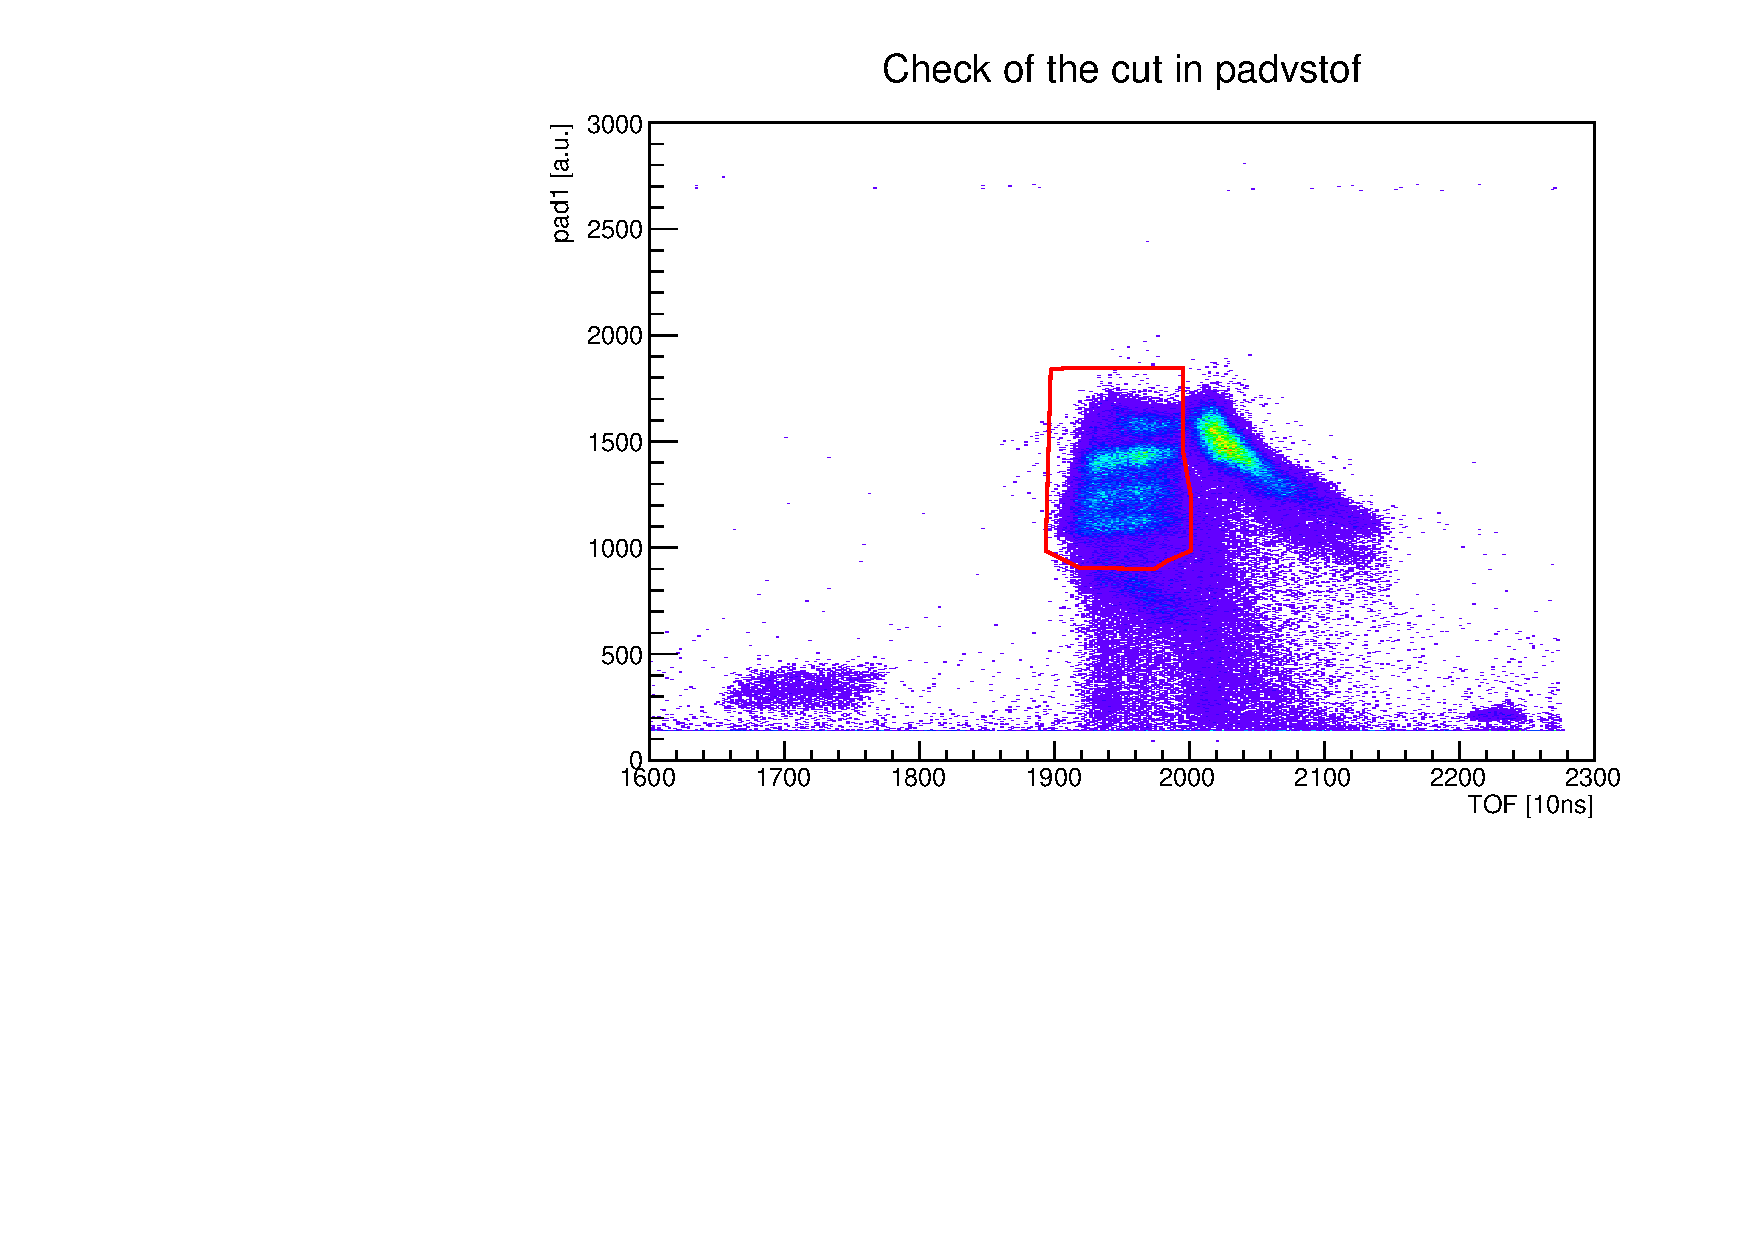
\includegraphics[width=\linewidth]{Figure/run2322-24Mg-pad1vstof.pdf}
	\caption{Pad1 vs TOF for a 24Mg run. Pad1 range 0,3000 bin 3000 - TOF range 1600,2300 bin 350}
	\label{fig:pad1vstof}
\end{figure}

\begin{figure}
	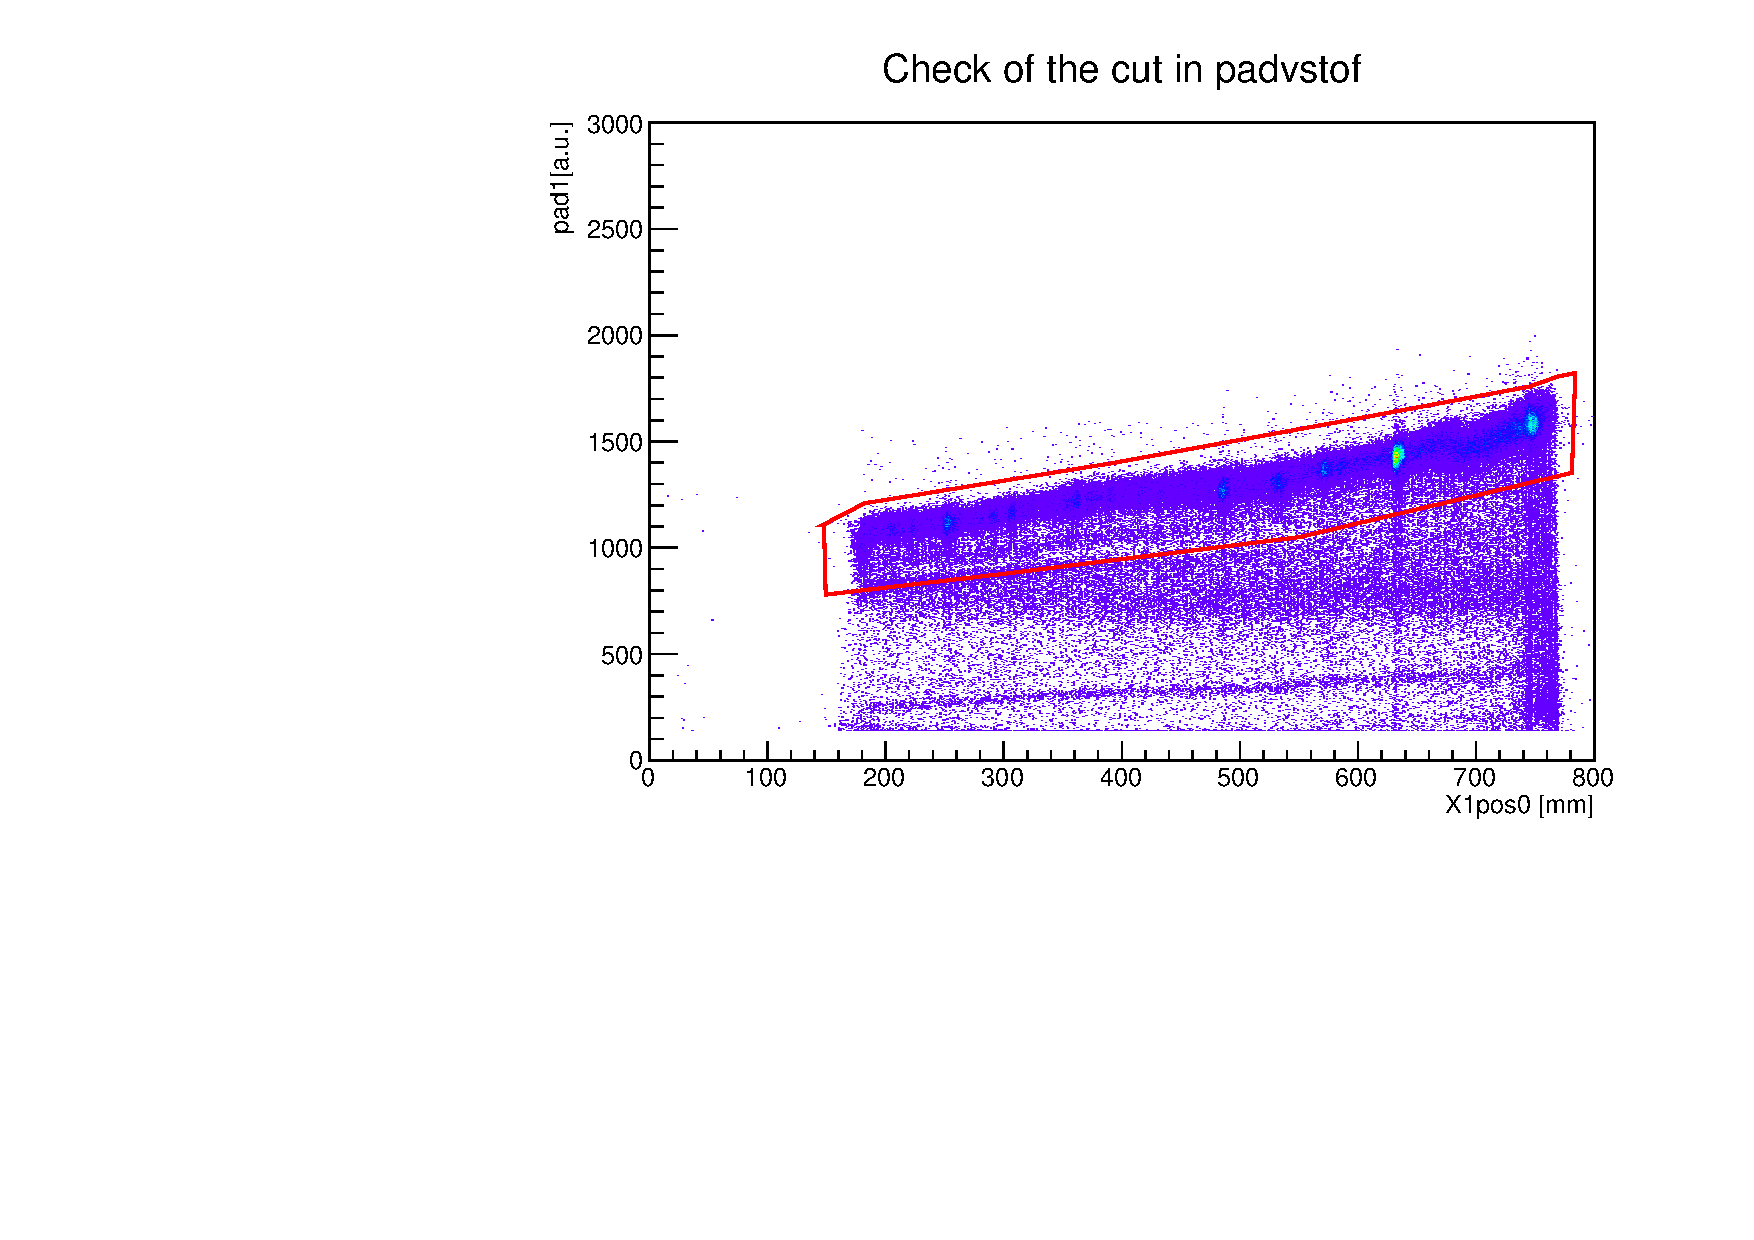
\includegraphics[width=\linewidth]{Figure/run2322-24Mg-pad1vsX1posO.pdf}
	\caption{Pad1 vs X1posO for a 24Mg run. Pad1 range 0,3000 bin 3000 - X1posO range 0,800 bin 800}
	\label{fig:pad1vsX1}
\end{figure}


\section{X1 alignment}

The X1pos spectra must also be aligned as described above.
\begin{enumerate}
	\item Use the code get$\_$peakpos.C to extract the X1 offsets. It extracts the X1 position of the most intense peak in the X1pos spectra for the list of runs given and it calculates the offsets of the peak position respect to the one in the first run of the list. The calculated offsets are saved in a .dat file. Edit the file to add "eof" at the end.
	\item Put the X1Offsets file in the Analyser folder.
	\item Modify the NrOfX1Offsets and XOffsetsFile in the config.cfg file.
	\item Run the Analyser and check that the offsets have been implemented. The variable "X1posO" in the rootTree is now the one corrected and "X1pos" is the uncorrected one.
\end{enumerate}

The aigment achevied in this procedure for the $^{24}Mg$ runs is 0.02mm.\\


\underline{Note}: for this procedure use the gate on pad1vstof, pad1vsX1, X1flag==0 and U1flag==0.

\section{Lineshape correction for X1Y1 and tofX1 matrix}
Due to optics aberrations the X1 value for events with different tof and Y1 is not the same. This distortion can be corrected by a lineshape function. 

The parameters for the correction can be calculated with the lineshapepar.C code.
The first step is to calculate the X1Y1 correction parameters. 
Figure \ref{fig:Y1vsX1_notcorr} shows the X1vsY1 spectrum before the correction. The red square indicates the peak that is used for the correction.
The code requires as inputs the X1 mean value of the selected peak (X1mean 633 for 24Mg runs) and the biny where to evaluate the fit (208-300 for 24Mg runs).
With these inputs the code calculated the X1 position for each biny slice and fit the results with a second order polynomial, see Fig. \ref{fig:Y1vsX1_fit}.\\
The second part of the code consists in the evaluation of the parameters for the X1vsTOF spectrum where now the X1 value is the one corrected for the Y1.
The procedure is the same for X1vsY1 case.
Figure \ref{fig:TOFvsX1_notcorr} and \ref{fig:TOFvsX1_notcorr_zoom} shows the spectrum before the correction: as one can clearly see the lines are not straight.
In this case the codes inputs are for the TOF mean value of the selected peak (TOFmean 1960 for 24Mg runs) and the biny where to evaluate the fit (10-90 for 24Mg runs). Figure \ref{fig:TOFvsX1_fit} shows the fit using a second order polynomial.\\
One has to notice that the lineshape correction is not constant with X1. For this reason the correction was calculated as
\begin{eqnarray}
X1CTOF&=&X1posO-[b1*(tof-TOFmean)+  \nonumber \\&+& b2*(tof-TOFmean)^2]*\dfrac{X1posO-X1ref}{X1mean-X1ref}
\end{eqnarray}

where X1ref refers to the position of the peak that doesn't need a correction (255 for 24Mg runs) and b1,b2 the coefficient of the X1vsTOF fit.\\
Figure \ref{fig:TOFvsX1_corr} shows the X1vsTOF spectrum after the correction. The line now are straight.


\begin{figure}
	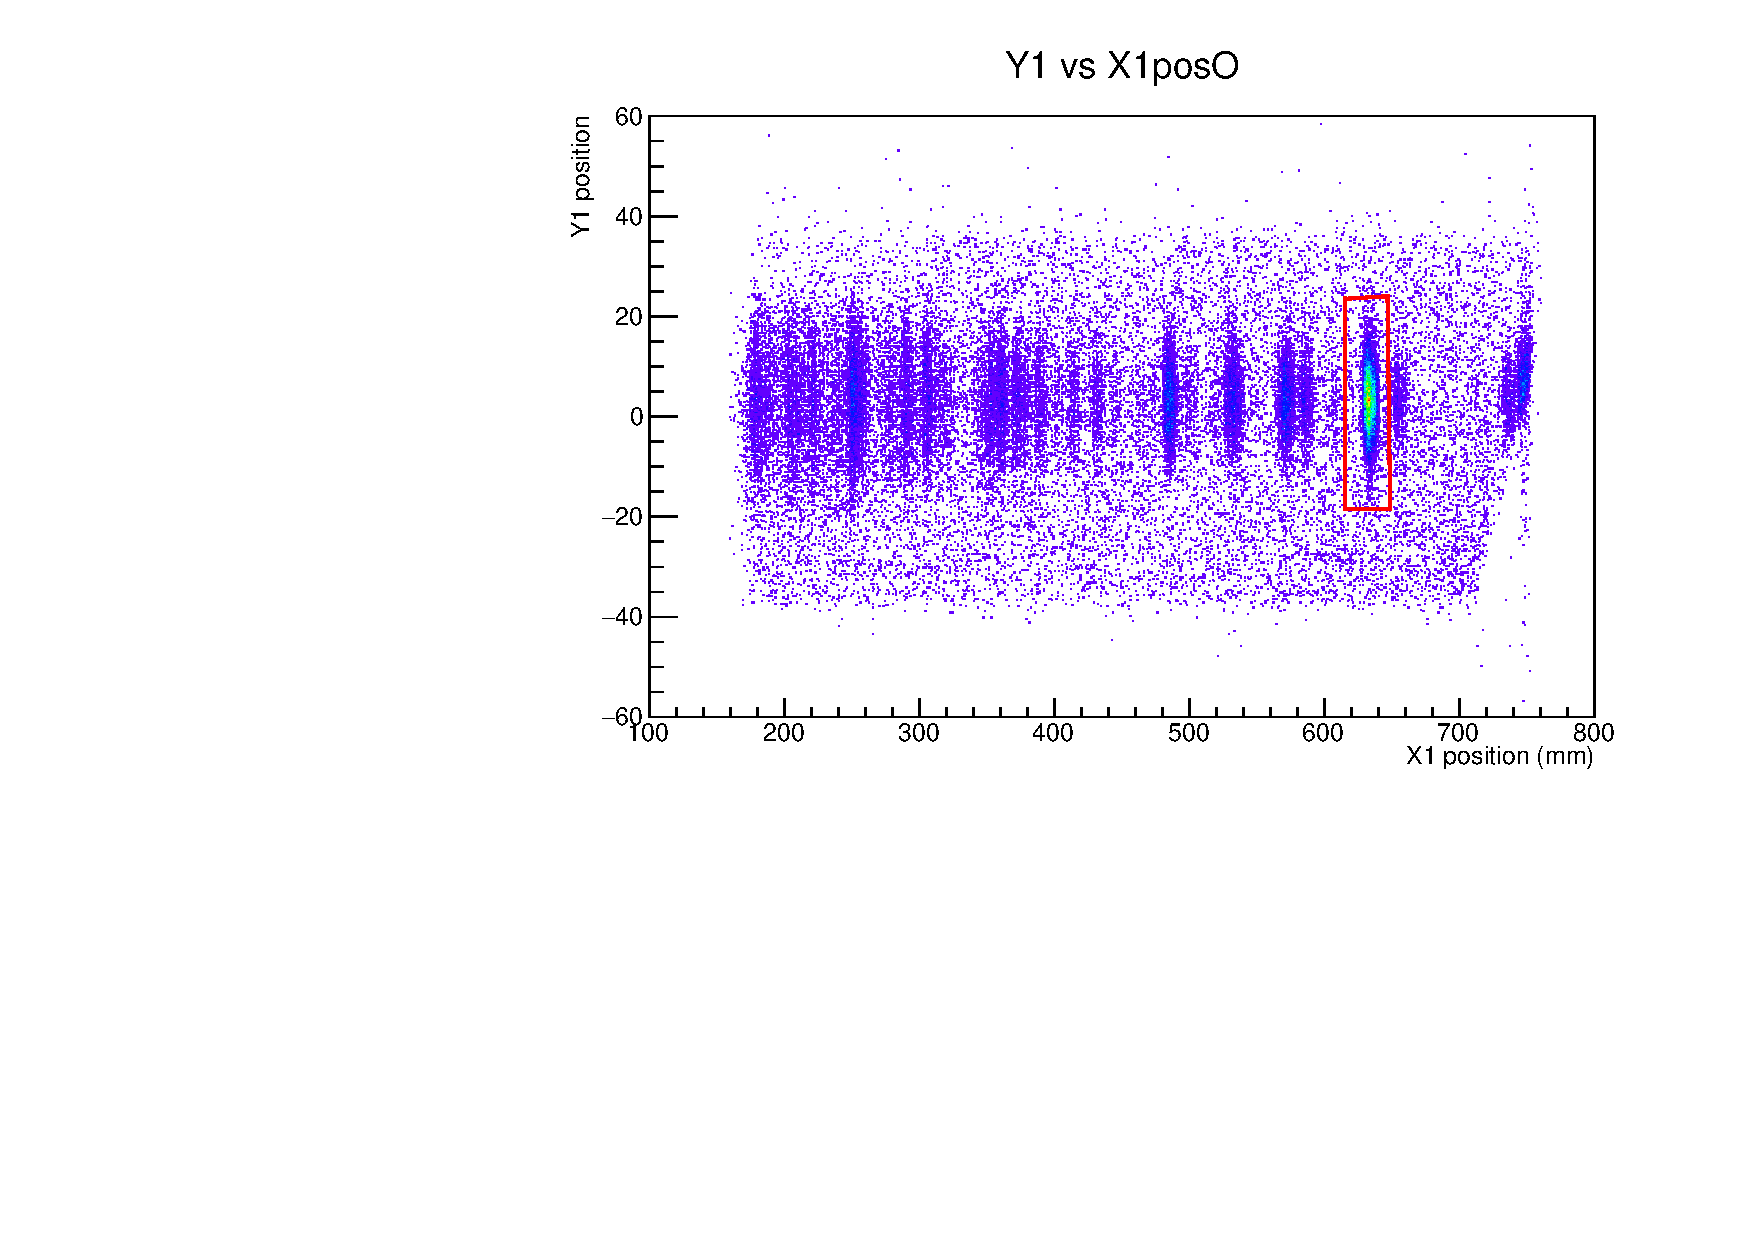
\includegraphics[width=\linewidth]{Figure/run2227-24Mg-lineshape-X1Y1-notcorr.pdf}
	\caption{Y1 vs X1posO for a 24Mg run before the lineshape correction. The red square indicates the peak used for the correction. Y1 range -60,60 bin 480 - X1posO range 0,800 bin 800}
	\label{fig:Y1vsX1_notcorr}
\end{figure}

\begin{figure}
	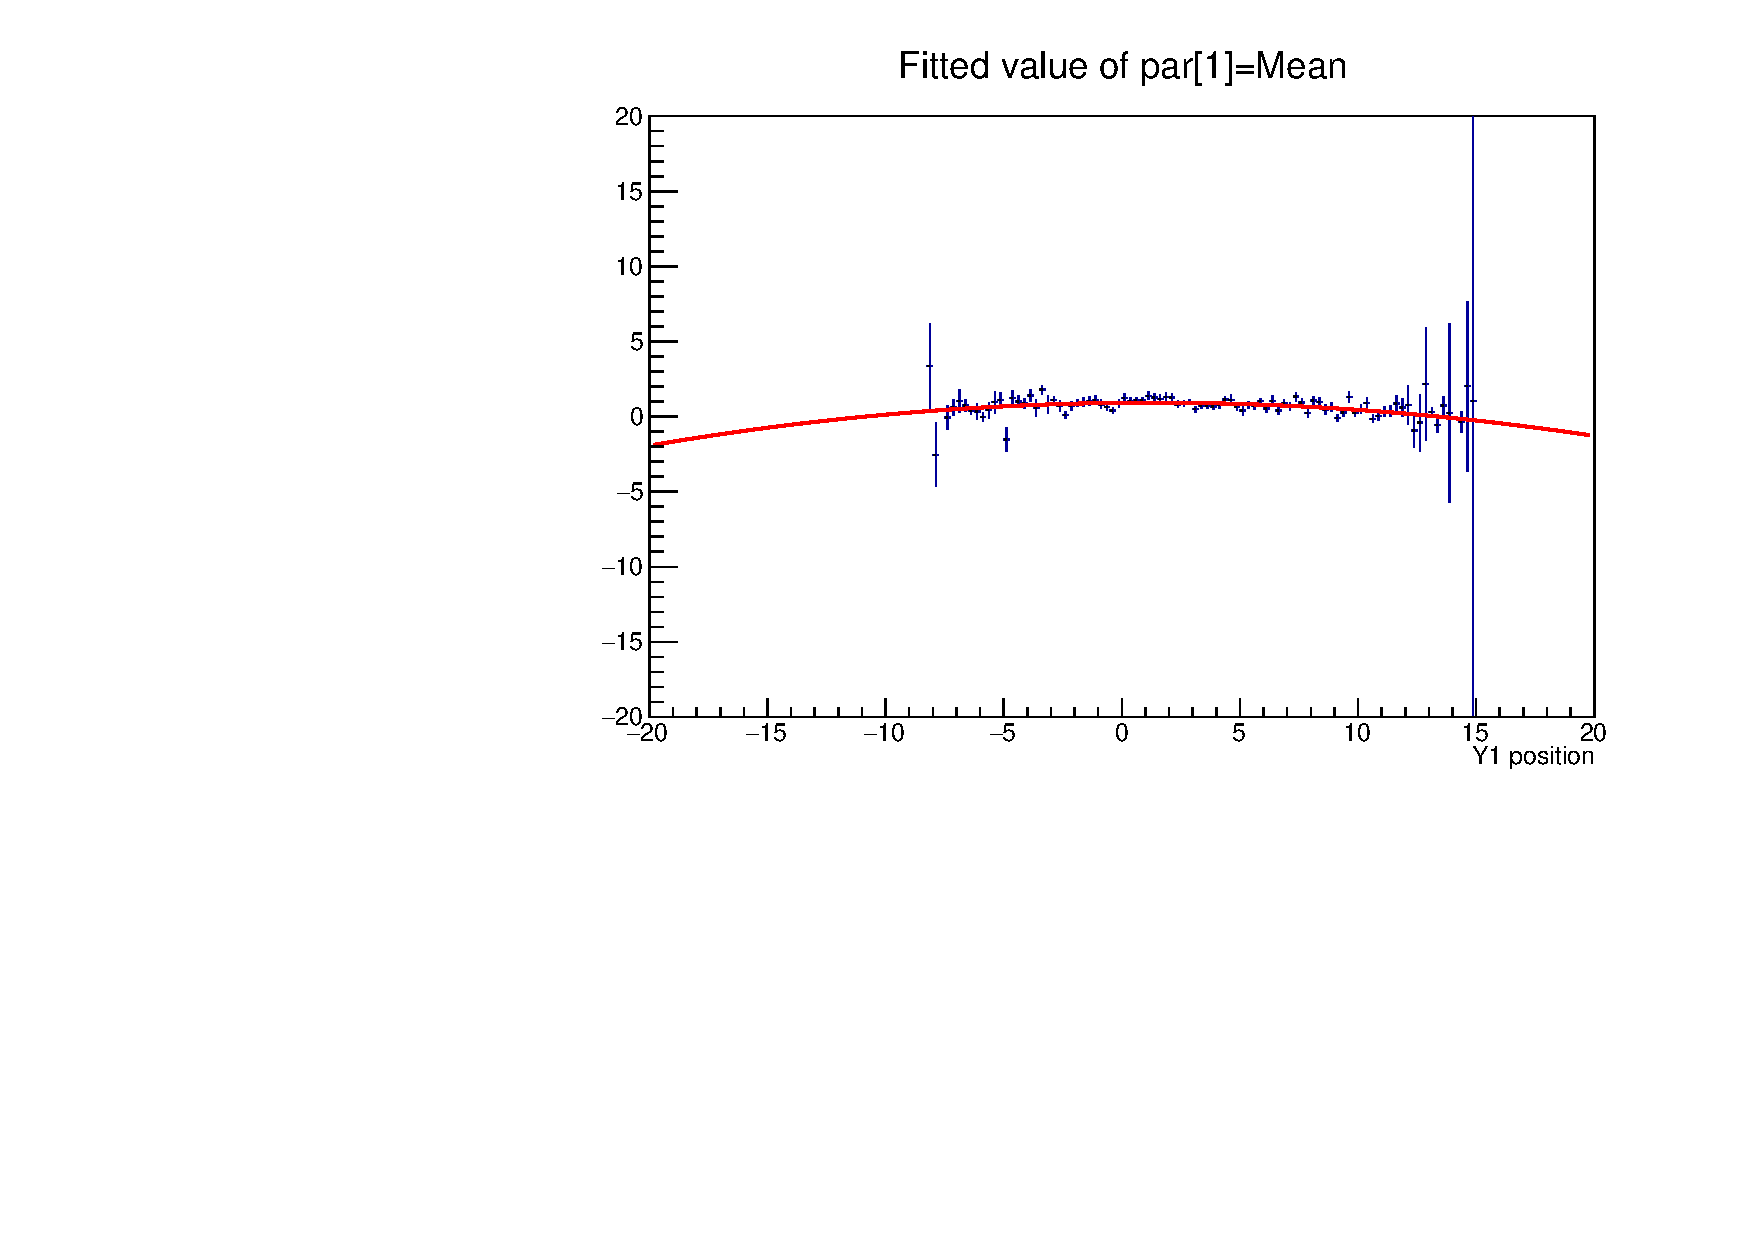
\includegraphics[width=\linewidth]{Figure/run2227-24Mg-lineshape-X1Y1-fit.pdf}
	\caption{Fit of the X1 positions for each Y1 bin. A second order polynomial was used.}
	\label{fig:Y1vsX1_fit}
\end{figure}

\begin{figure}
	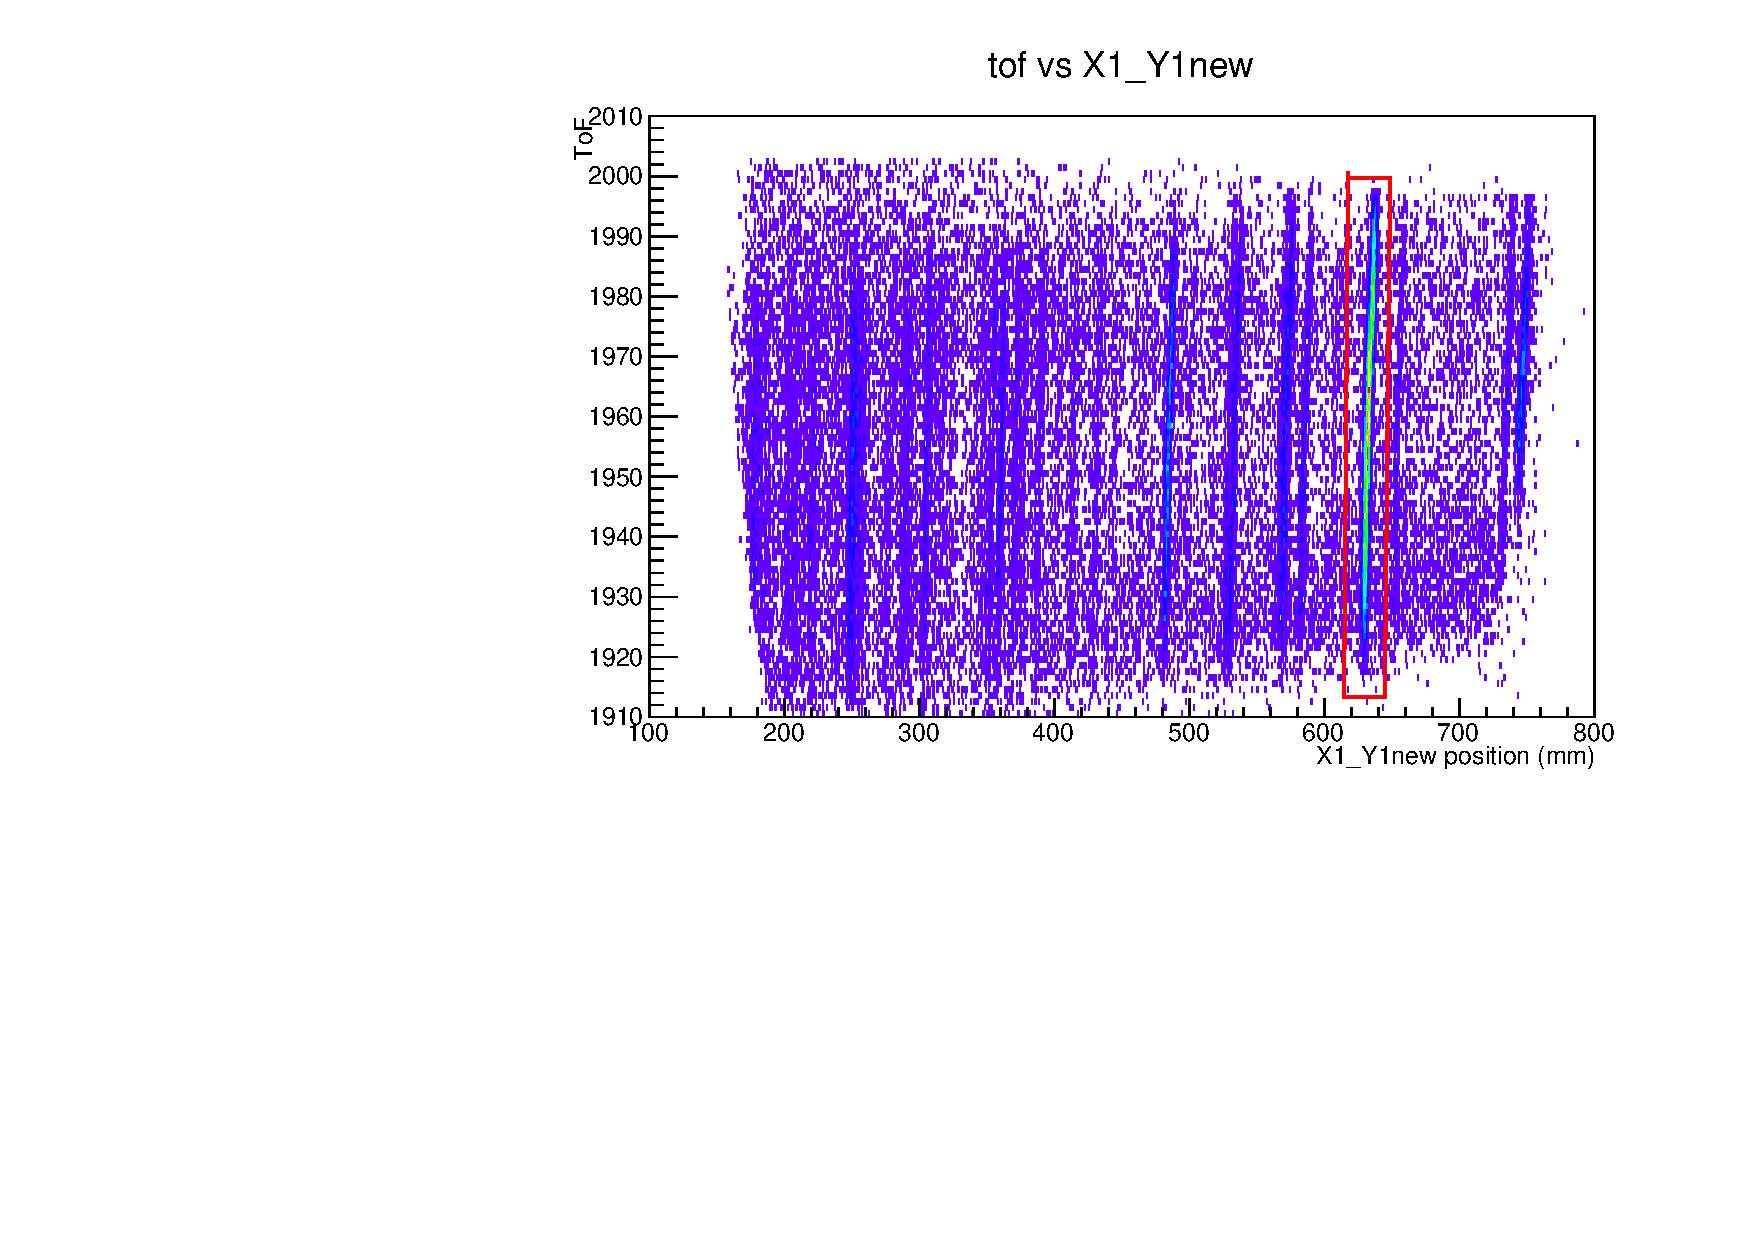
\includegraphics[width=\linewidth]{Figure/run2227-24Mg-lineshape-X1TOF-notcorr.pdf}
	\caption{TOF vs X1posO for a 24Mg run before the lineshape correction. The red square indicates the peak used for the correction.}
	\label{fig:TOFvsX1_notcorr}
\end{figure}

\begin{figure}
	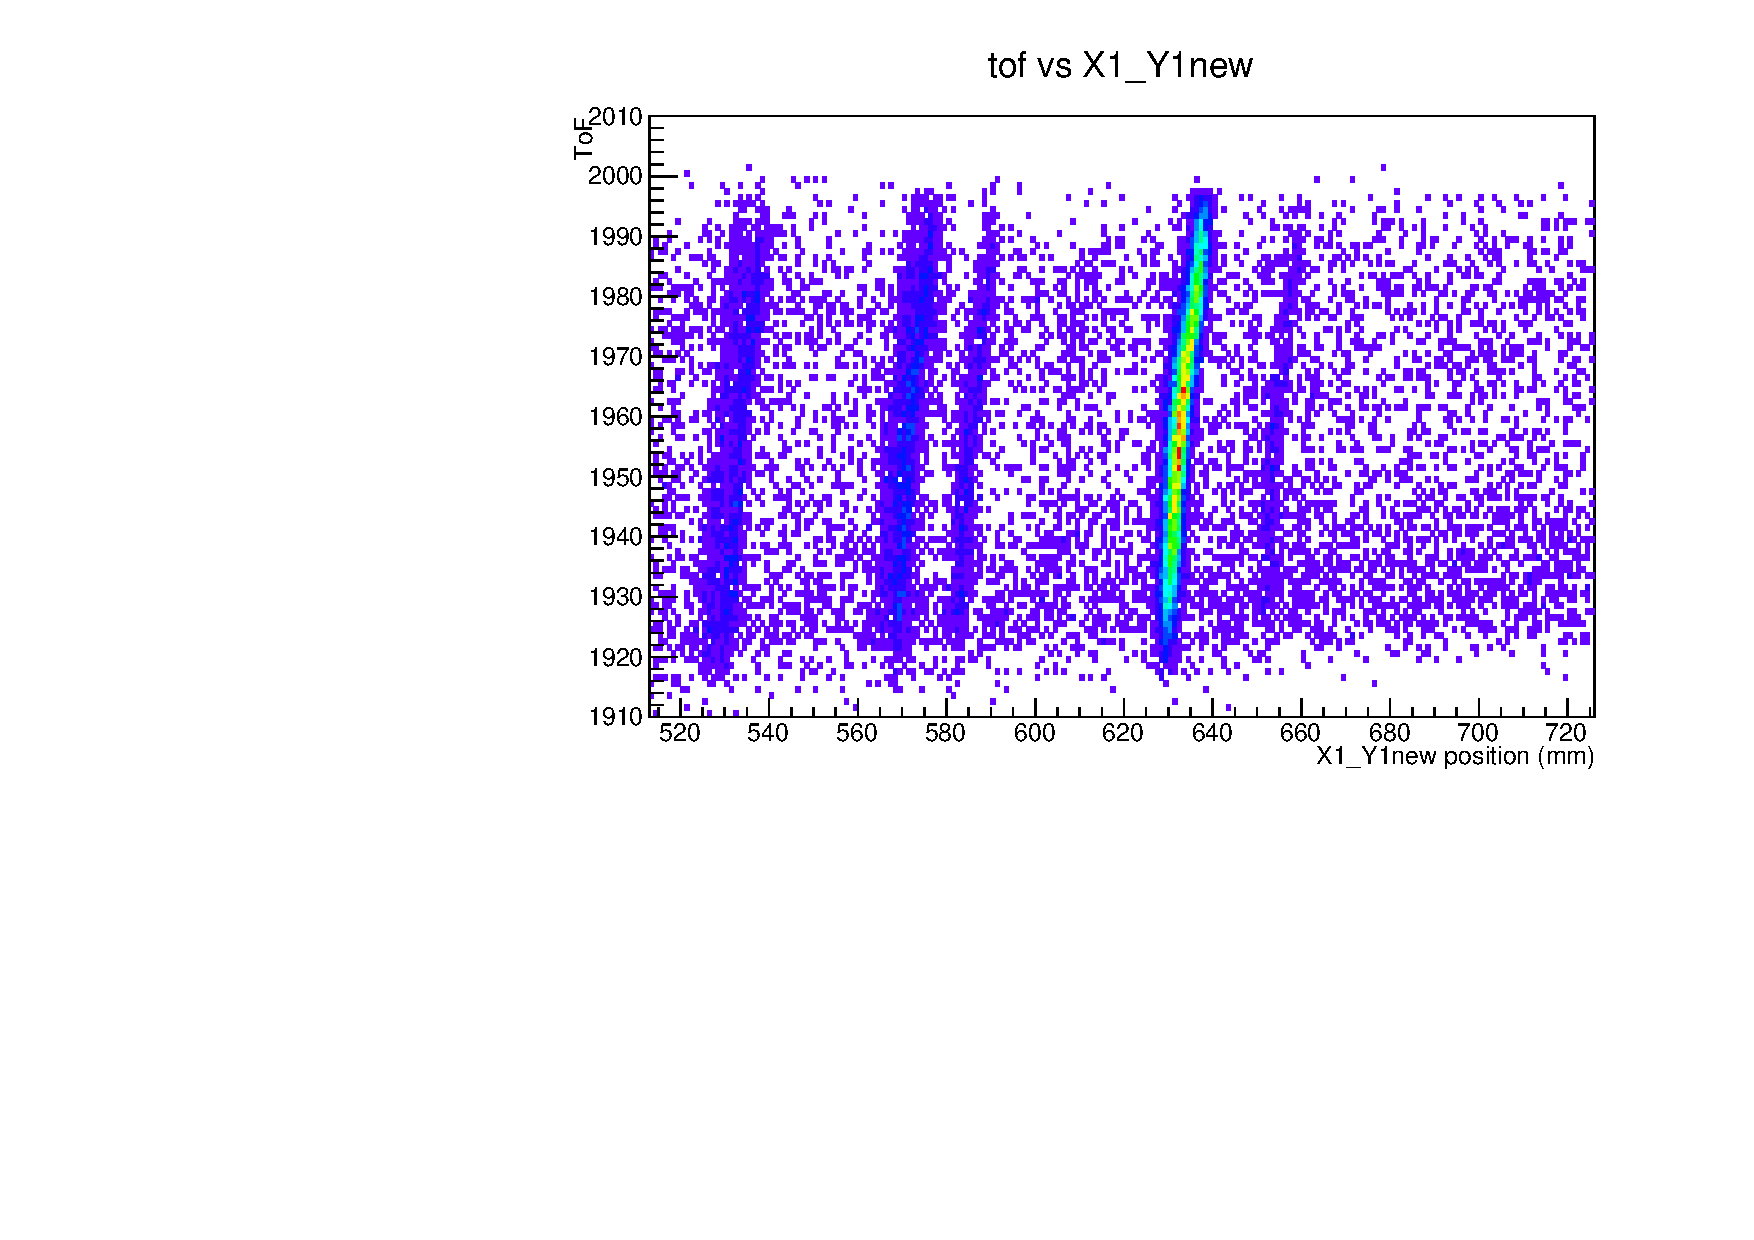
\includegraphics[width=\linewidth]{Figure/run2227-24Mg-lineshape-X1TOF-notcorr-zoom.pdf}
	\caption{Zoom of the TOF vs X1posO for a 24Mg run before the lineshape correction.}
	\label{fig:TOFvsX1_notcorr_zoom}
\end{figure}

\begin{figure}
	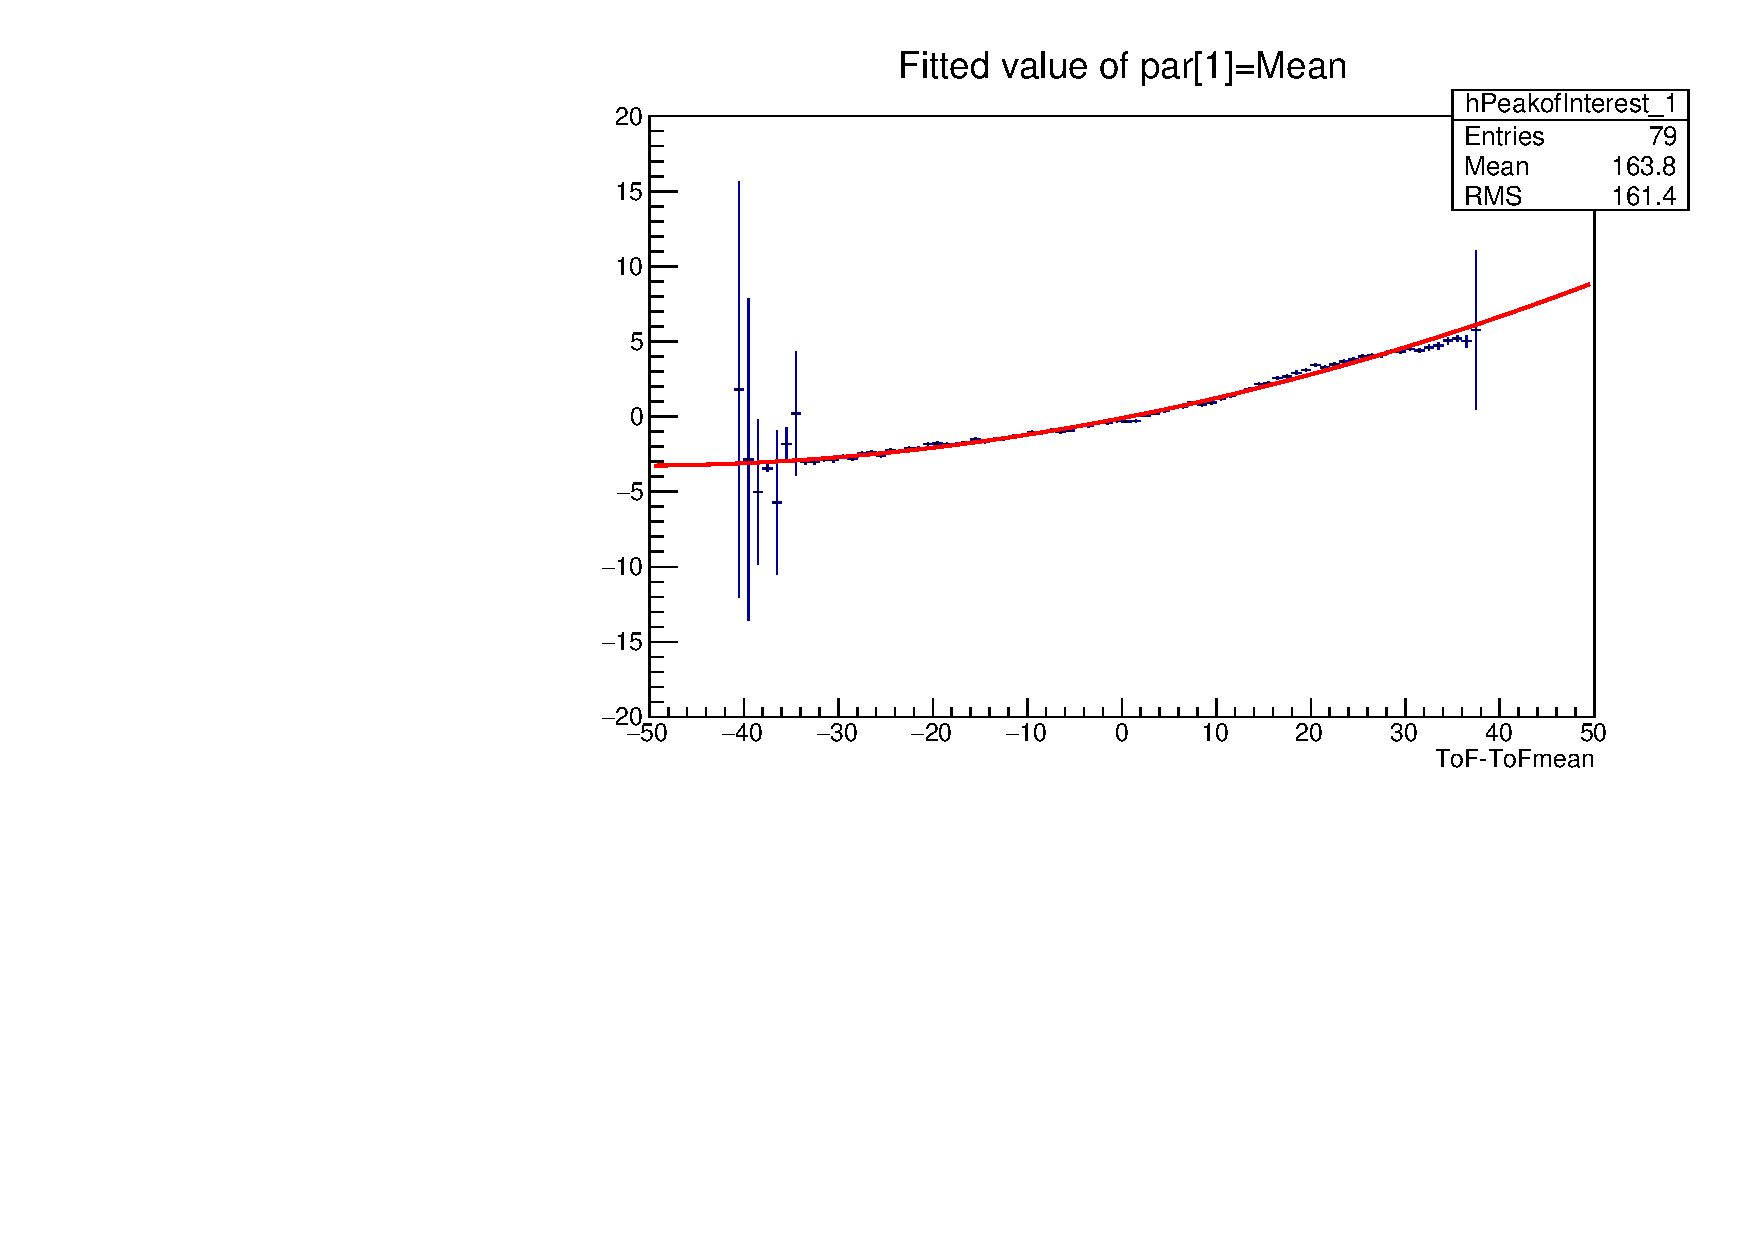
\includegraphics[width=\linewidth]{Figure/run2227-24Mg-lineshape-X1TOF-fit.pdf}
	\caption{Fit of the X1 positions for each TOF bin. A second order polynomial was used.}
	\label{fig:TOFvsX1_fit}
\end{figure}

\begin{figure}
	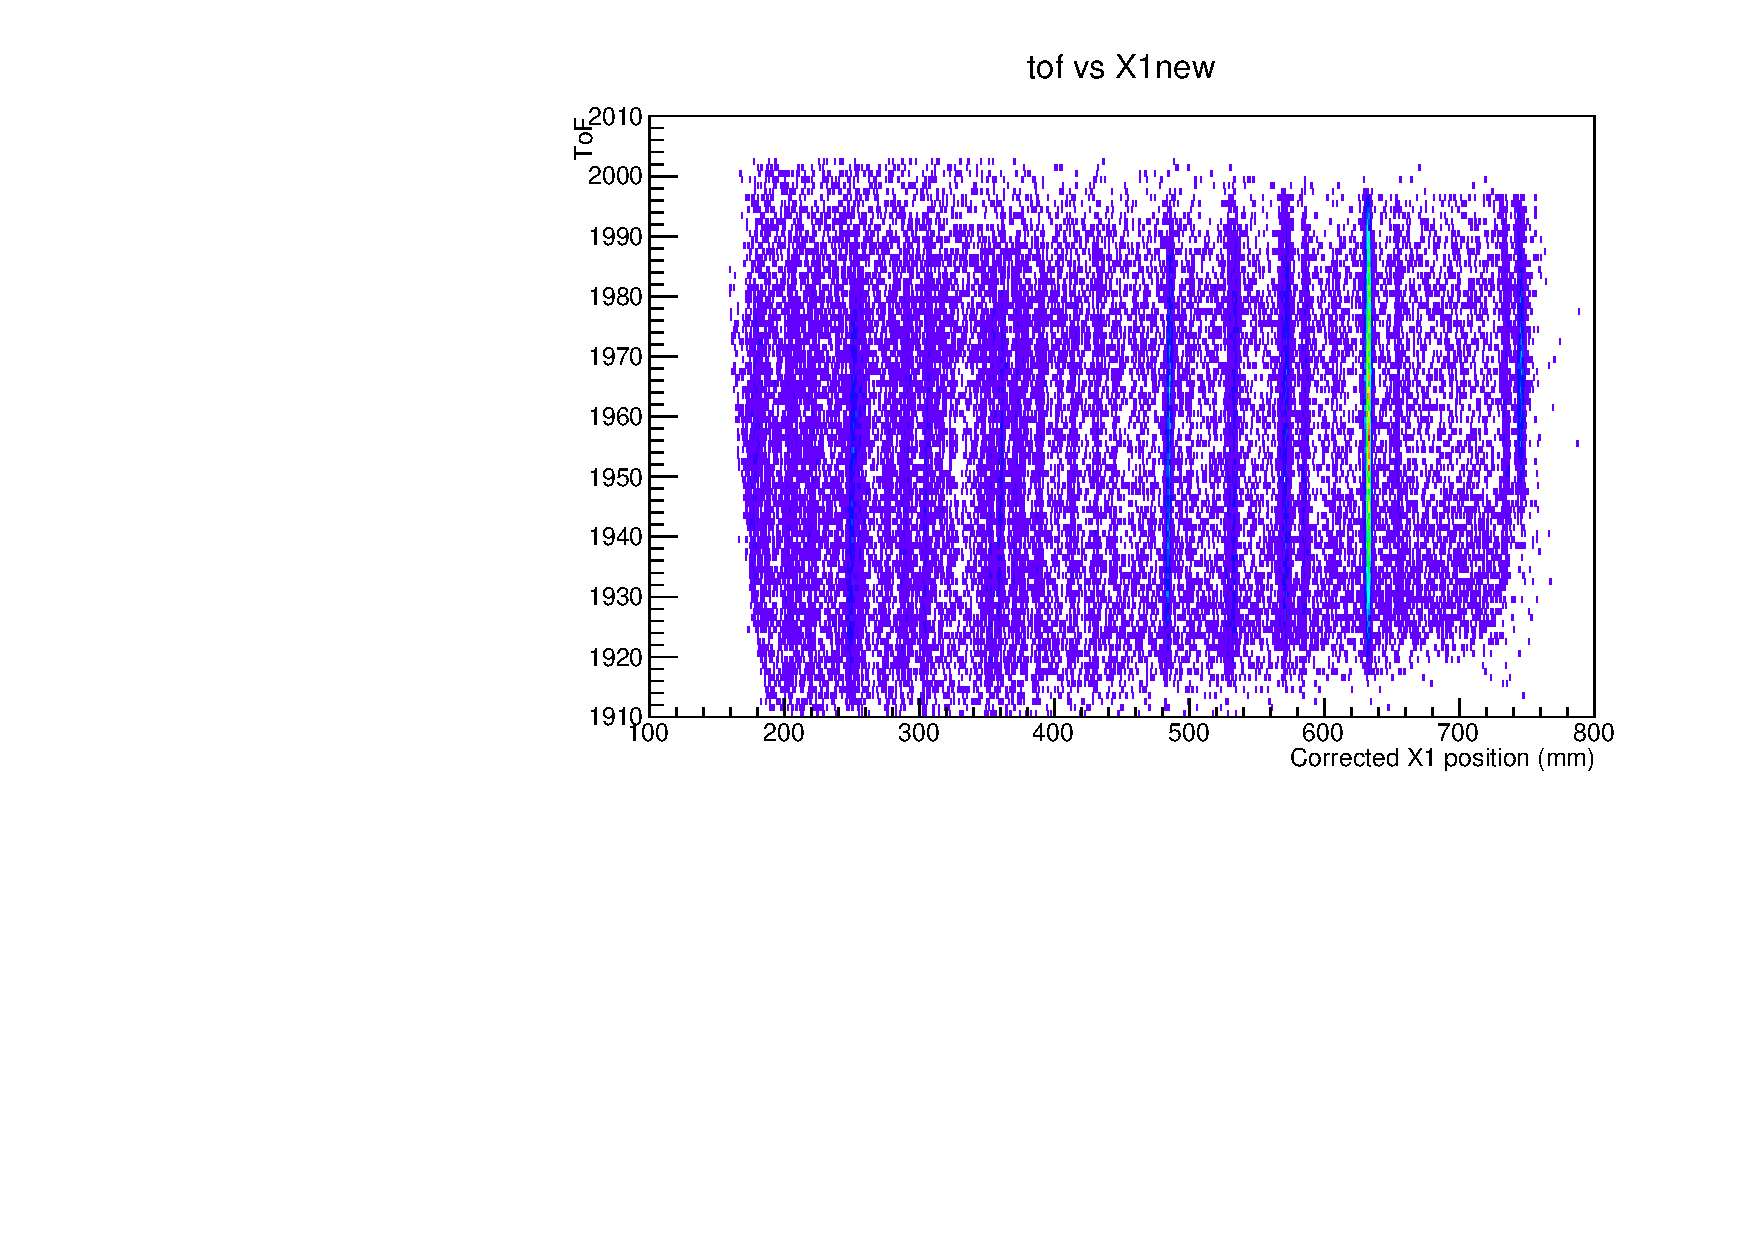
\includegraphics[width=\linewidth]{Figure/run2227-24Mg-lineshape-X1TOF-corr.pdf}
	\caption{TOF vs X1posO for a 24Mg run after the lineshape correction. The line are now straight.}
	\label{fig:TOFvsX1_corr}
\end{figure}



\chapter{K600 Calibration}
The procedure to calibrate the K600 spectra consists of the following points:
\begin{enumerate}
	\item Select the calibration target and extract the positions of the peak of interest.
	\item Use the code SPANC to calculate the product of QB$\rho$ for the corresponding excitation energy of the peak selected in point 1. \\To do so you need to know the beam energy, the scattering angle, the target thickness and the excitation energies. Note that the QB$\rho$ units that SPANC use are [ekGcm] which, with the proper unit conversion, is the same of [CTm]. 
	\item Once you have the peak position and the corresponding QB$\rho$ value, the parameters of a polynomial fit must be extracted, see Fig. \ref{fig:ExvsQBrho_fit}. The order of the polynomial must be chosen to better fit the data (usually a second order is enough).
	
	\begin{figure}
		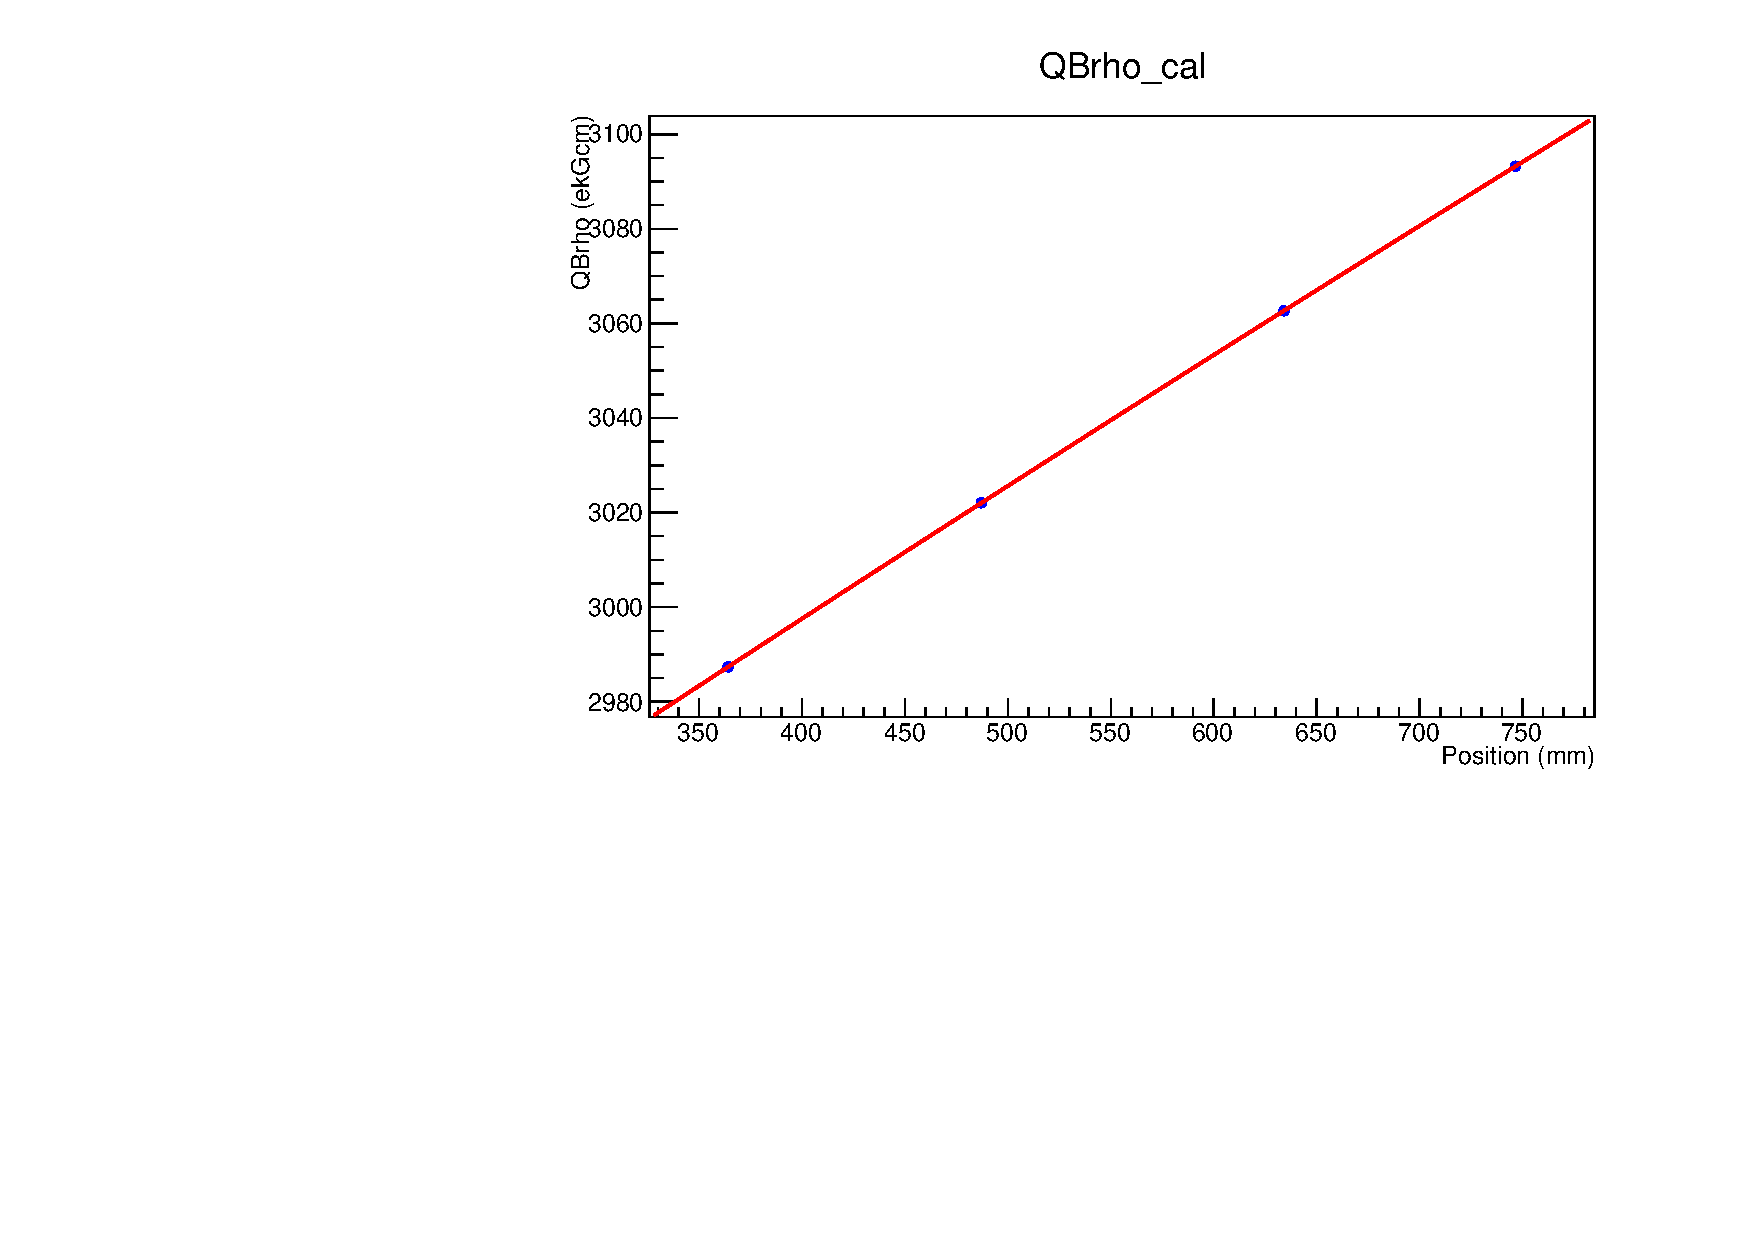
\includegraphics[width=\linewidth]{Figure/QBrho_24Mgcalib.pdf}
		\caption{Fit of the QB$\rho$ vs E$_x$ values for selected peaks in 24Mg. A second order polynomial was used.}
		\label{fig:ExvsQBrho_fit}
	\end{figure}
	
	\item The QB$\rho$ parameters must be implemented in the configuration file (config.cfg) of the analyser to calculate the corresponding QB$\rho$ value for each event. The parameters must be inserted in the "RigidityCalibration" section. The function for the calculation is implemented in the FocalPlane.c code under the name "CalcQBrho" and a new leaf named "rigidity3" is added in the rootTree (see Fig.\ref{fig:rigidity3_24Mg}).
	
		\begin{figure}
			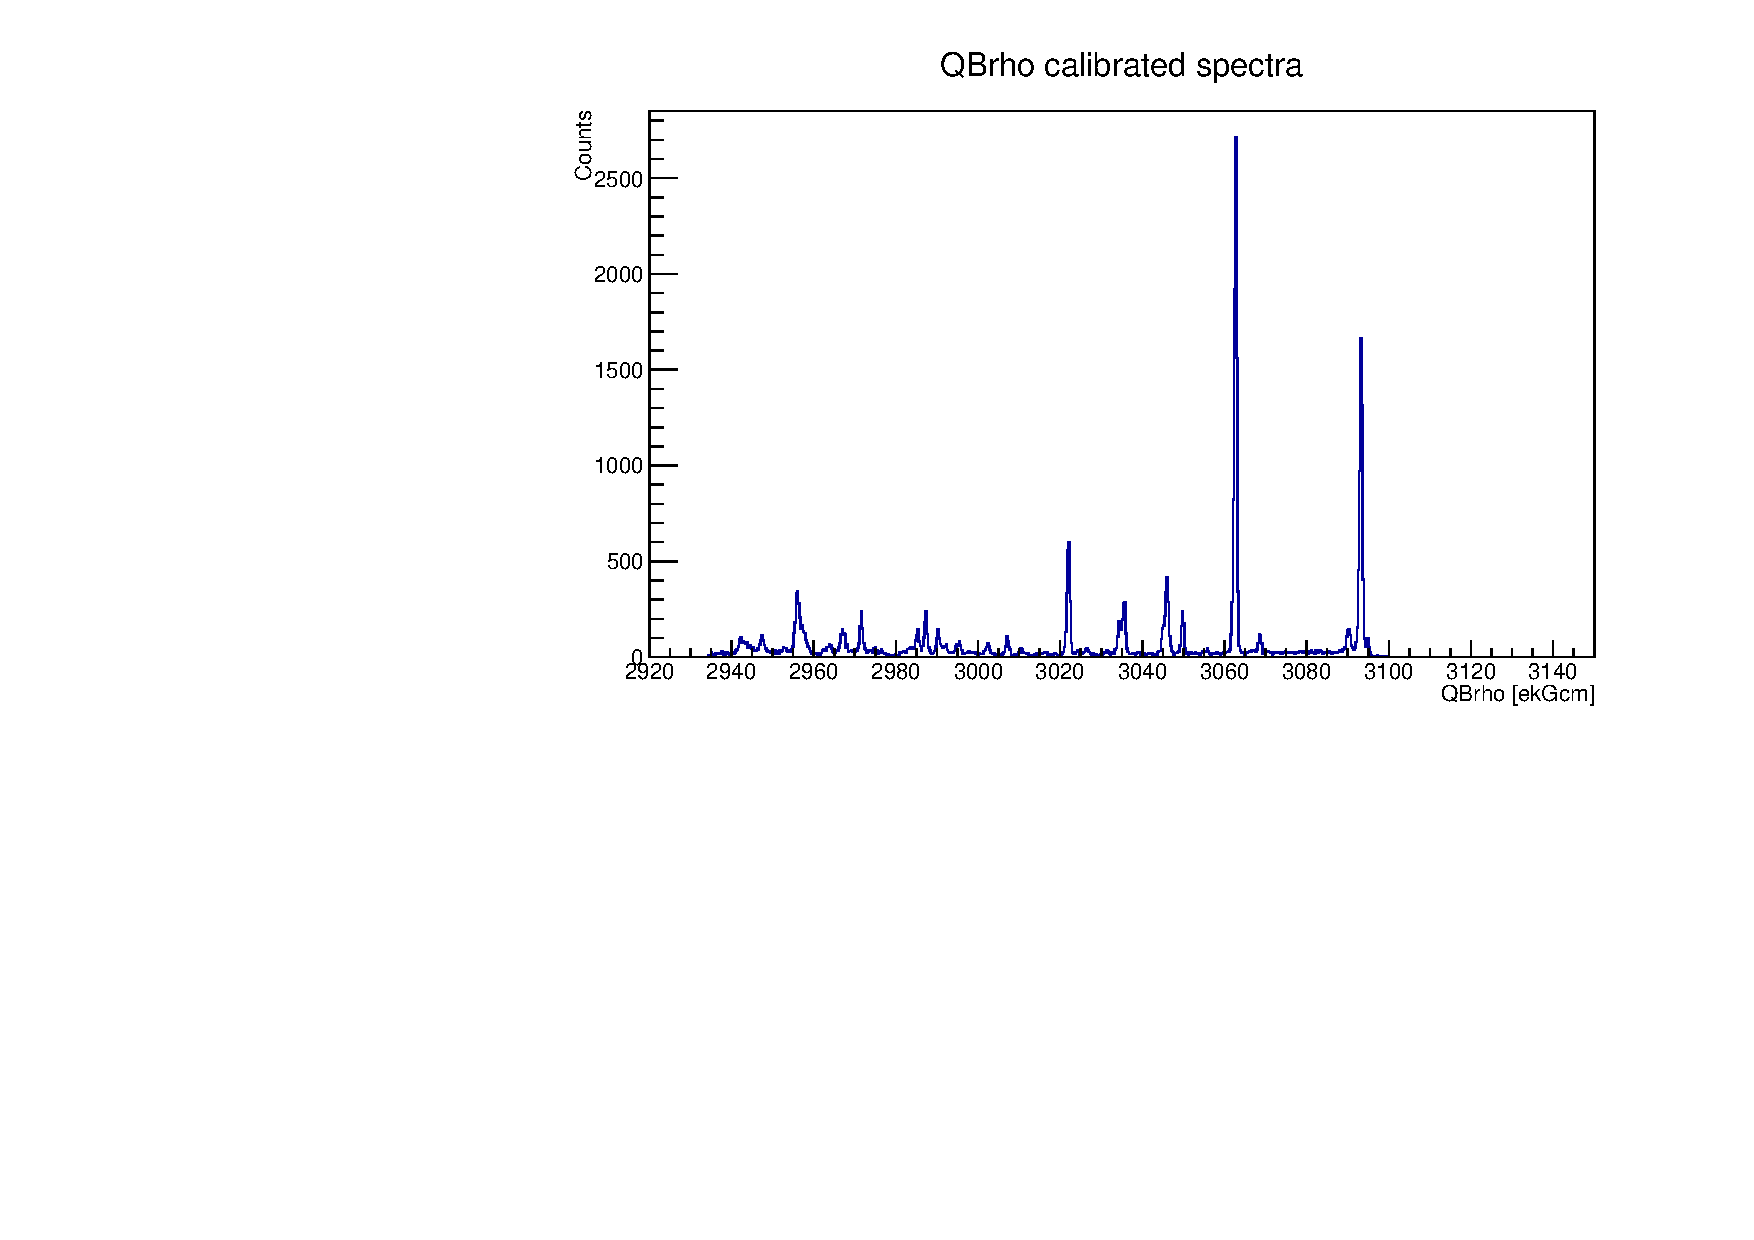
\includegraphics[width=\linewidth]{Figure/run02464_rigidity3.pdf}
			\caption{Rigidity spectrum for 24Mg.}
			\label{fig:rigidity3_24Mg}
		\end{figure}
	
	\item From the QB$\rho$ values the excitation energy spectrum can be extracted by using a proper relativistic kinematics calculation. This procedure is already implemented in the FocalPlane.c through the function "CalcEx". The only thing that the user should do is to add the mass value (the one used by SPANC), if the reaction is inelastic scattering and the scattering angle in the section "Kinematics related issues" of the config.cfg file.
	\item A new leaf for the excitation energy value will be created in the rootTree under the name "Ex", see Fig. .
\end{enumerate}

		\begin{figure}
			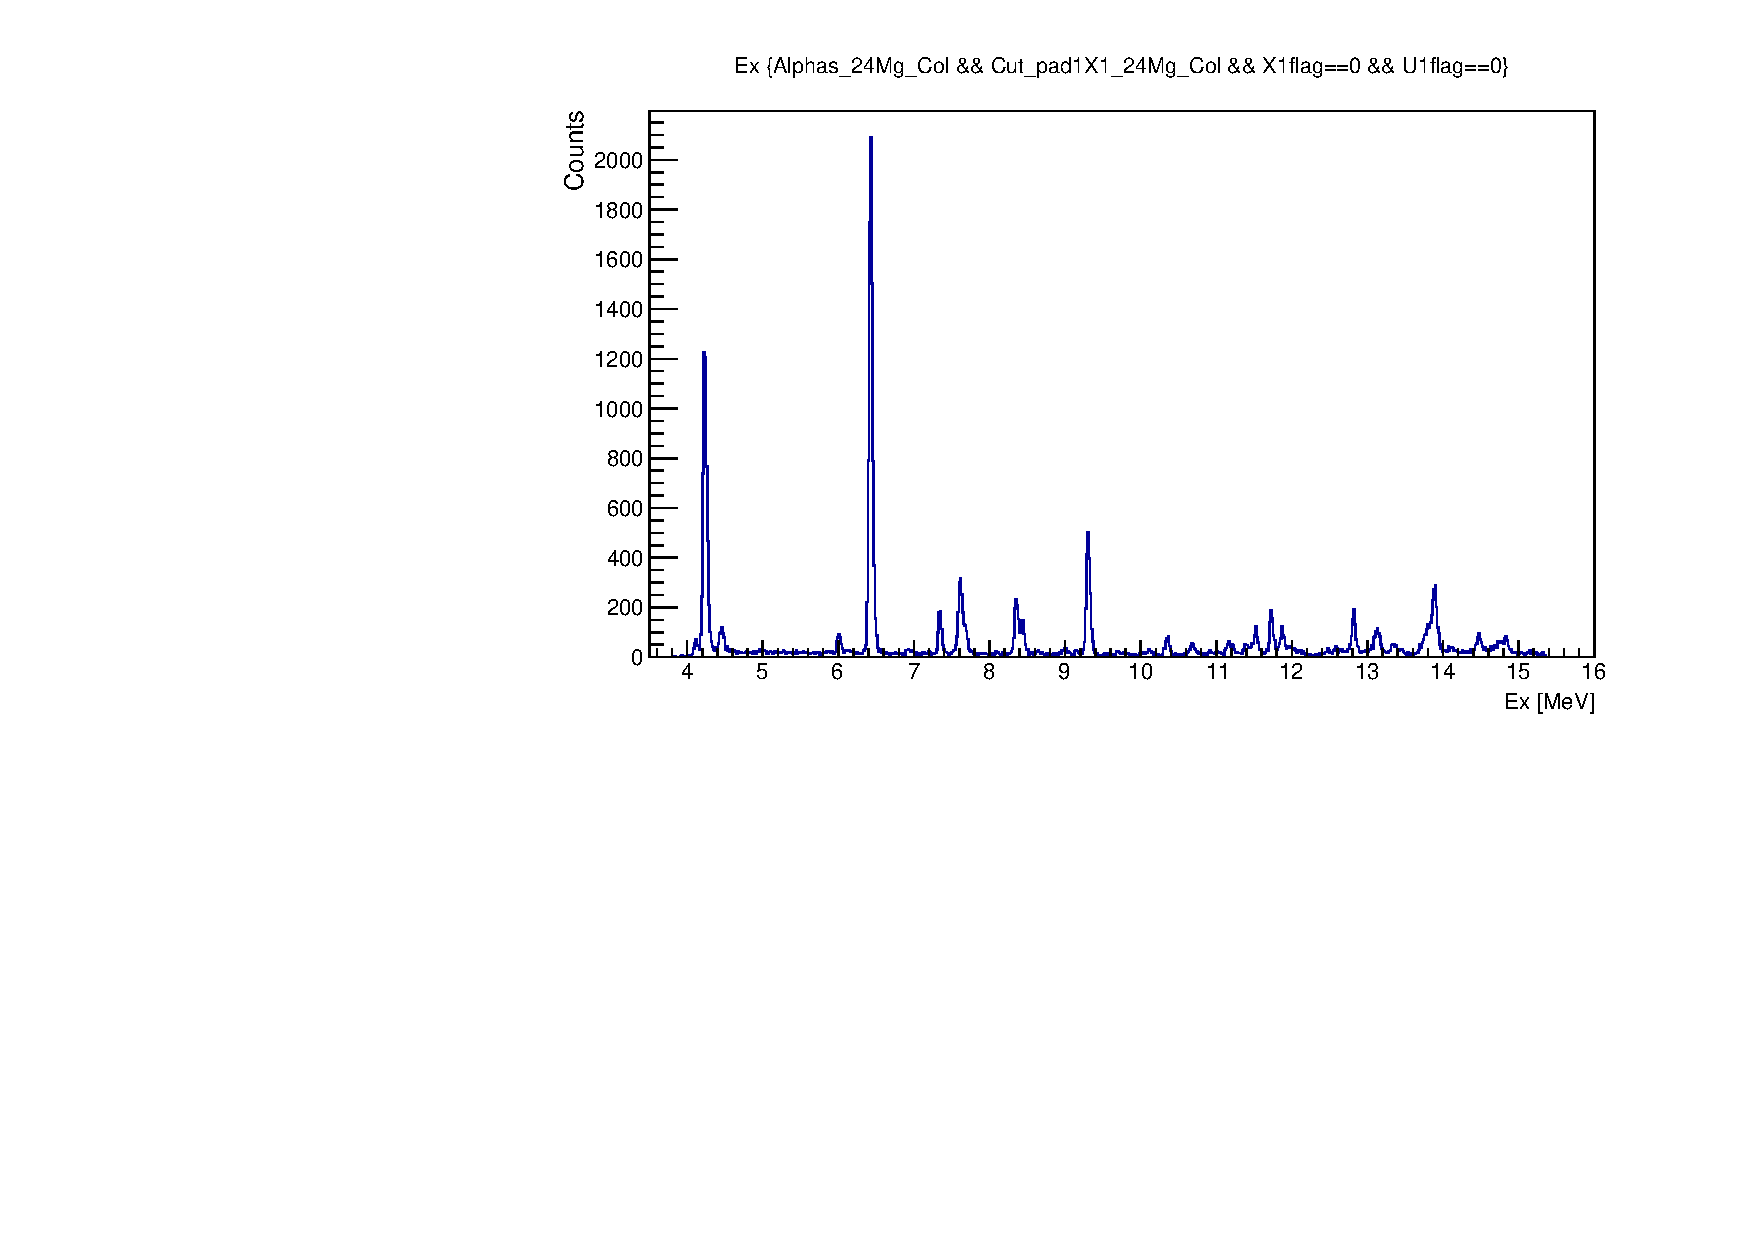
\includegraphics[width=\linewidth]{Figure/run02464_Ex_allgates.pdf}
			\caption{Excitation energy spectrum for 24Mg. Gates on PID and PadvsX1 are implemented.}
			\label{fig:Ex_24Mg}
		\end{figure}

It has to be noticed that this calibration procedure has been tested so far only in the case of inelastic scattering data. \par
This method for excitation energy calculation is particular important when the target of interest doesn't show distinct peaks that can be used for the calibration. In this case a well known target with several peaks in the region of interest (usually $^{24/26}$Mg) can be use to extract the calibration coefficients. These coefficients will then be translated in the experiment target by the kinematics calculation.\par
In the sections below a detailed description of the units conversion for QB$\rho$ and the relativistic kinematics calculation are reported.

\section{Rigidity - Units conversion}

From SPANC: QB$\rho$[$e\cdot kG\cdot cm$]\\
\begin{eqnarray}
QB\rho[C\cdot T\cdot m] &=& p[\frac{kg\cdot m}{s}] \nonumber\\
p[\frac{eV}{c}] &=& p[\frac{kg\cdot m}{s}]\cdot\frac{c}{e}\nonumber\\
QB\rho[C\cdot T\cdot m] &=& QB\rho[e\cdot kG\cdot cm]\cdot\frac{e}{10^3}\nonumber\\
p[\frac{MeV}{c}] &=& QB\rho[e\cdot kG\cdot cm]\cdot\frac{c}{10^3}\cdot\frac{1}{10^6} \nonumber\\
\mathbf{p[\frac{MeV}{c}]} &\mathbf{=}& \mathbf{QB\rho[e\cdot kG\cdot cm]\cdot\frac{c}{10^9}}
\end{eqnarray}
The units conversion coefficient are already implemented in the PR251 version of the analyser. 

\section{Two-body kinematics calculation in laboratory frame}

\begin{figure}
	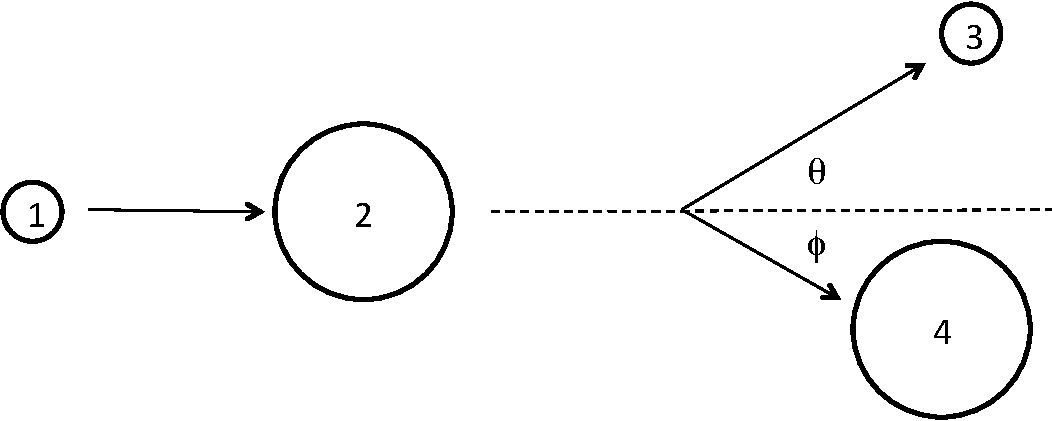
\includegraphics[width=\linewidth]{Figure/scattering.pdf}
	\caption{Kinematic of a nuclear reaction}
	\label{fig:scattering}
\end{figure}


Energy conservation law:
\begin{equation}
E_1 + E_2 = E_3 + E_4 + E_x
\label{eq:energy}
\end{equation}
Momentum conservation law:
\begin{eqnarray}
p_1 &=& p_3\cos\theta + p_4\cos\phi\nonumber\\
0 &=& p_3\sin\theta - p_4\sin\phi
\label{eq:momentum}
\end{eqnarray}

note: $E =T + mc^2$, $E^2 = p^2c^2 + m^2c^4$ and $Q = (m_1 + m_2 - m_3 - m_4)c^2$.

If we do the square of equations \ref{eq:momentum} 
\begin{eqnarray}
(p_1- p_3\cos\theta)^2 &=&  p_4^2\cos^2\phi\nonumber\\
p_3^2\sin^2\theta &=& p_4^2\sin^2\phi\nonumber
\end{eqnarray}
and we sum them, we obtain:
\begin{eqnarray}
p_1^2 - 2p_1p_3\cos\theta + p_3^2\cos^2\theta + p_3^2\sin^2\theta &=&  p_4^2(\sin^2\phi +\cos^2\phi)\nonumber\\
p_1^2 + p_3^2 - 2p_1p_3\cos\theta &=& p_4^2
\label{eq:p4}
\end{eqnarray}
From equation \ref{eq:energy}
\begin{eqnarray}
T_1 + m_1c^2 + m_2c^2 &=& T_3 + m_3c^2 + T_4 + m_4c^2 + E_x\\
E_x &=& T_1 - T_3 - T_4 + m_1c^2 + m_2c^2 - m_3c^2 - m_4c^2 \nonumber\\
E_x &=& T_1 - T_3 - T_4 + Q
\end{eqnarray}

\begin{eqnarray}
T_1 &=& T_{beam}\nonumber\\
T_3 &=& \sqrt{p^2_3c^2+m_3^2c^4} - m_3c^2\nonumber\\
T_4 &=& \sqrt{p^2_4c^2+m_4^2c^4} - m_4c^2
\end{eqnarray}

using equation \ref{eq:p4}
\begin{equation}
T_4 = \sqrt{p_1^2c^2 + p_3^2c^2 - 2p_1p_3c^2\cos\theta+m_4^2c^4} - m_4c^2
\end{equation}

\begin{equation}
E_x = T_1 -\sqrt{p^2_3c^2+m_3^2c^4} + m_3c^2 - \sqrt{p_1^2c^2 + p_3^2c^2 - 2p_1p_3c^2\cos\theta+m_4^2c^4} + m_4c^2 + Q
\end{equation}

For the inelastic scatting case Q = 0 and we use natural units where c=1, we obtain:
\begin{equation}
\mathbf{E_x = T_1 -\sqrt{p^2_3+m_3^2} + m_3 - \sqrt{p_1^2 + p_3^2 - 2p_1p_3\cos\theta+m_4^2} + m_4}
\end{equation}
\\



\section{Background subtraction}

To minimized the background, the spectrometer was operated in vertical focus mode.This means that the events of interest are focused around $y_{fp}$ = 0 and the background coming from target and beam is evenly spread in the vertical direction.\\
Figure \ref{fig:Y1vsEx_vertline} shows the Y1 vs Ex matrix for 24Mg target. As it can be seen the events of interests are focused around Y=0. The black line shows a region with no peaks were the shape of the background was estimated. The Y1 projection of this region is shown in Fig. \ref{fig:Y1projection_bkg} where it can be seen that the background is not constant along the vertical range. For this reason the subtracted background must be properly normalised. Figure \ref{fig:Y1vsEx_orizline} shows the Y1vsEx matrix for 24Mg target. The subtracted background is highlight by the dashed black lines (Y1 bins from -35 to -25) and showed in Fig. \ref{fig:Ex_bkg}. The dashed red lines indicates the good events (bins from -20 to 20) from which the background has been subtracted.
The normalization factor was extracted from Fig. \ref{fig:Y1projection_bkg} as follow:

\begin{eqnarray}
norm_factor = \frac{integral_in_binrange(-20,20)}{integral_in_binrange(-35,-25)}
\end{eqnarray},

The normalised background extracted from Fig. \ref{fig:Ex_bkg} is fitted and subtracted from the excitation energy spectrum. Figure \ref{fig:Ex_bkgandnobkg} shows the comparison of the Ex spectrum before (blue) and after (red) the subtraction.

		\begin{figure}
			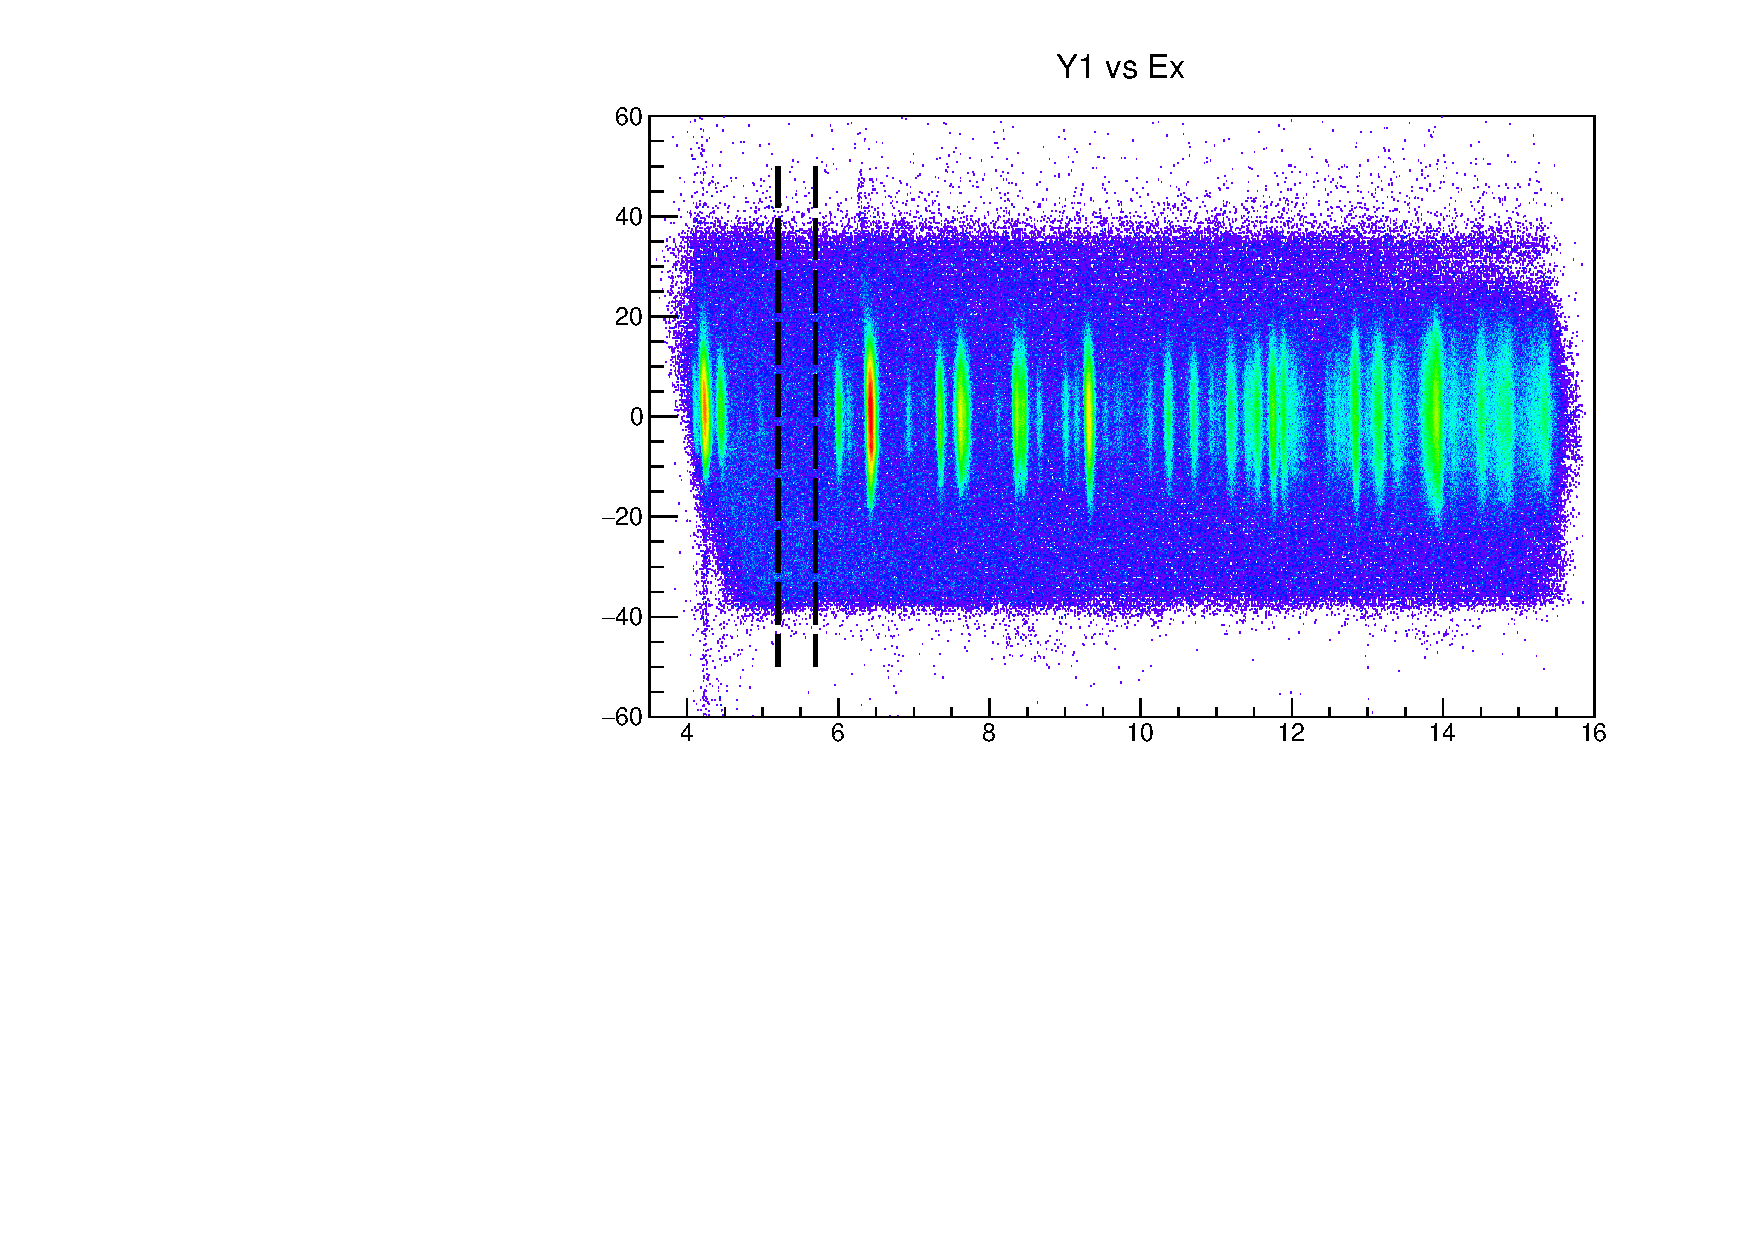
\includegraphics[width=\linewidth]{Figure/bkg/Chained_24Mg_Y1vsEx_2.pdf}
			\caption{Y1 vs Ex matrix for 24Mg. The dashed black lines highlight the region where the shape of the background was estimated.}
			\label{fig:Y1vsEx_vertline}
		\end{figure}
		
		\begin{figure}
			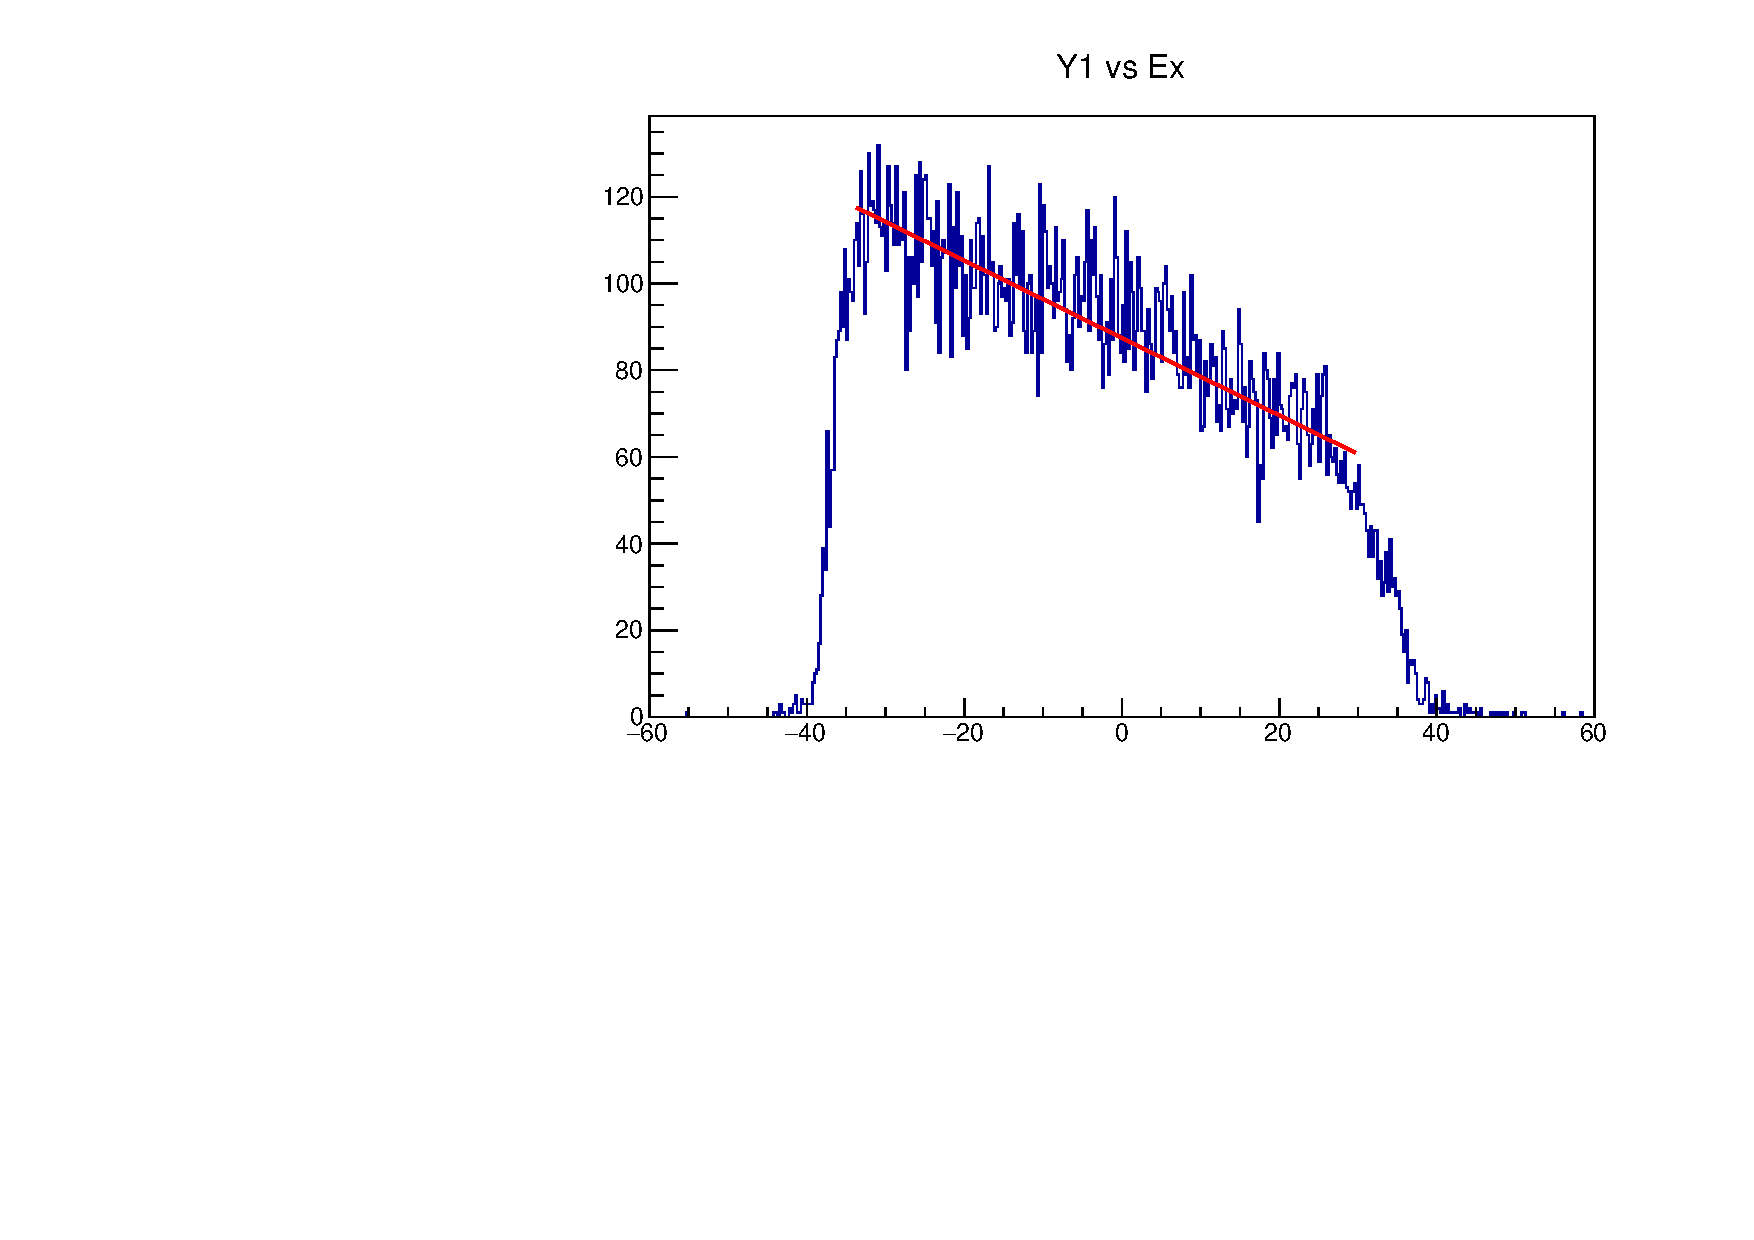
\includegraphics[width=\linewidth]{Figure/bkg/Chained_24Mg_Y1_projection.pdf}
			\caption{Y1 spectrum of the region selected in Fig. \ref{fig:Y1vsEx_vertline}. The background is not constant over the vertical range.}
			\label{fig:Y1projection_bkg}
		\end{figure}

		\begin{figure}
			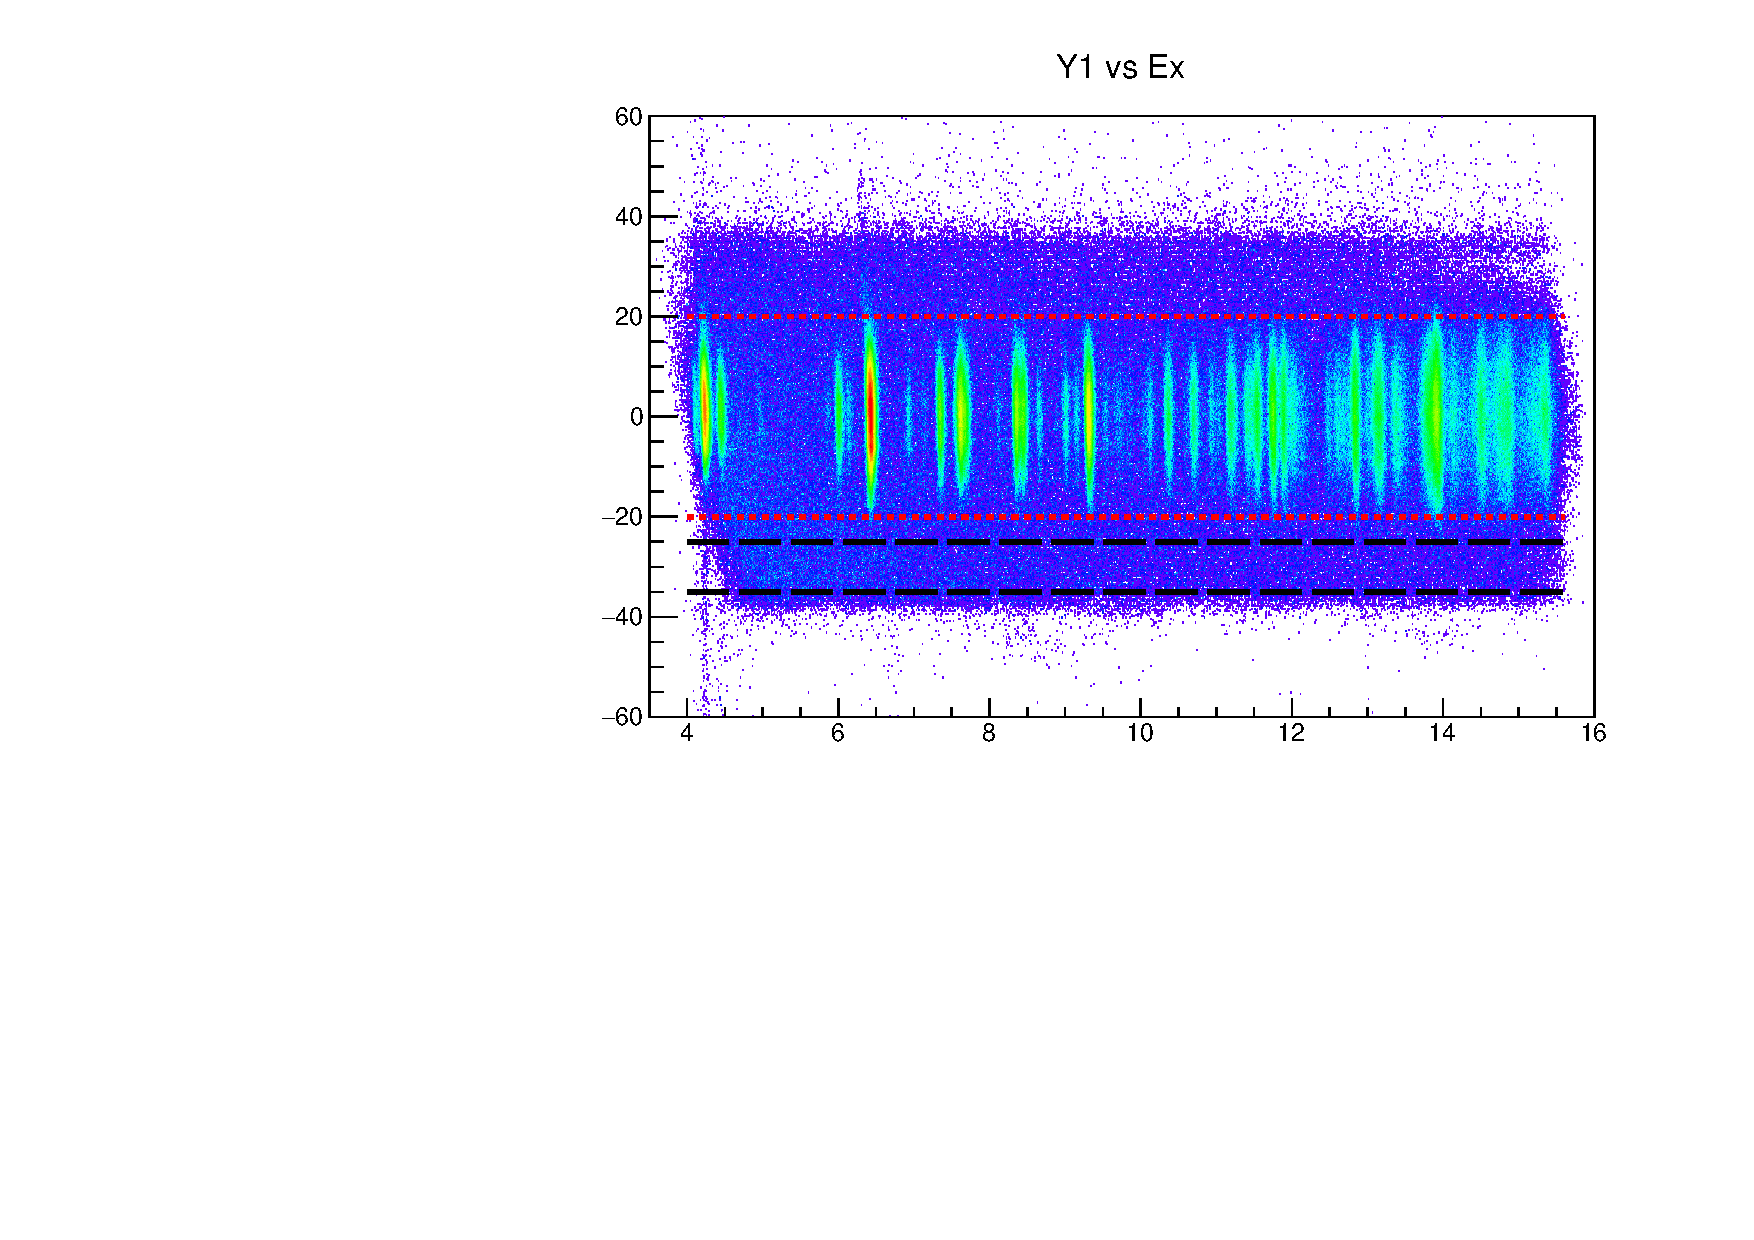
\includegraphics[width=\linewidth]{Figure/bkg/Chained_24Mg_Y1vsEx.pdf}
			\caption{Y1 vs Ex matrix for 24Mg. The subtracted background is highlight by the dashed black lines. The dashed red lines indicates the good events from which the background has been subtracted.}
			\label{fig:Y1vsEx_orizline}
		\end{figure}

		\begin{figure}
			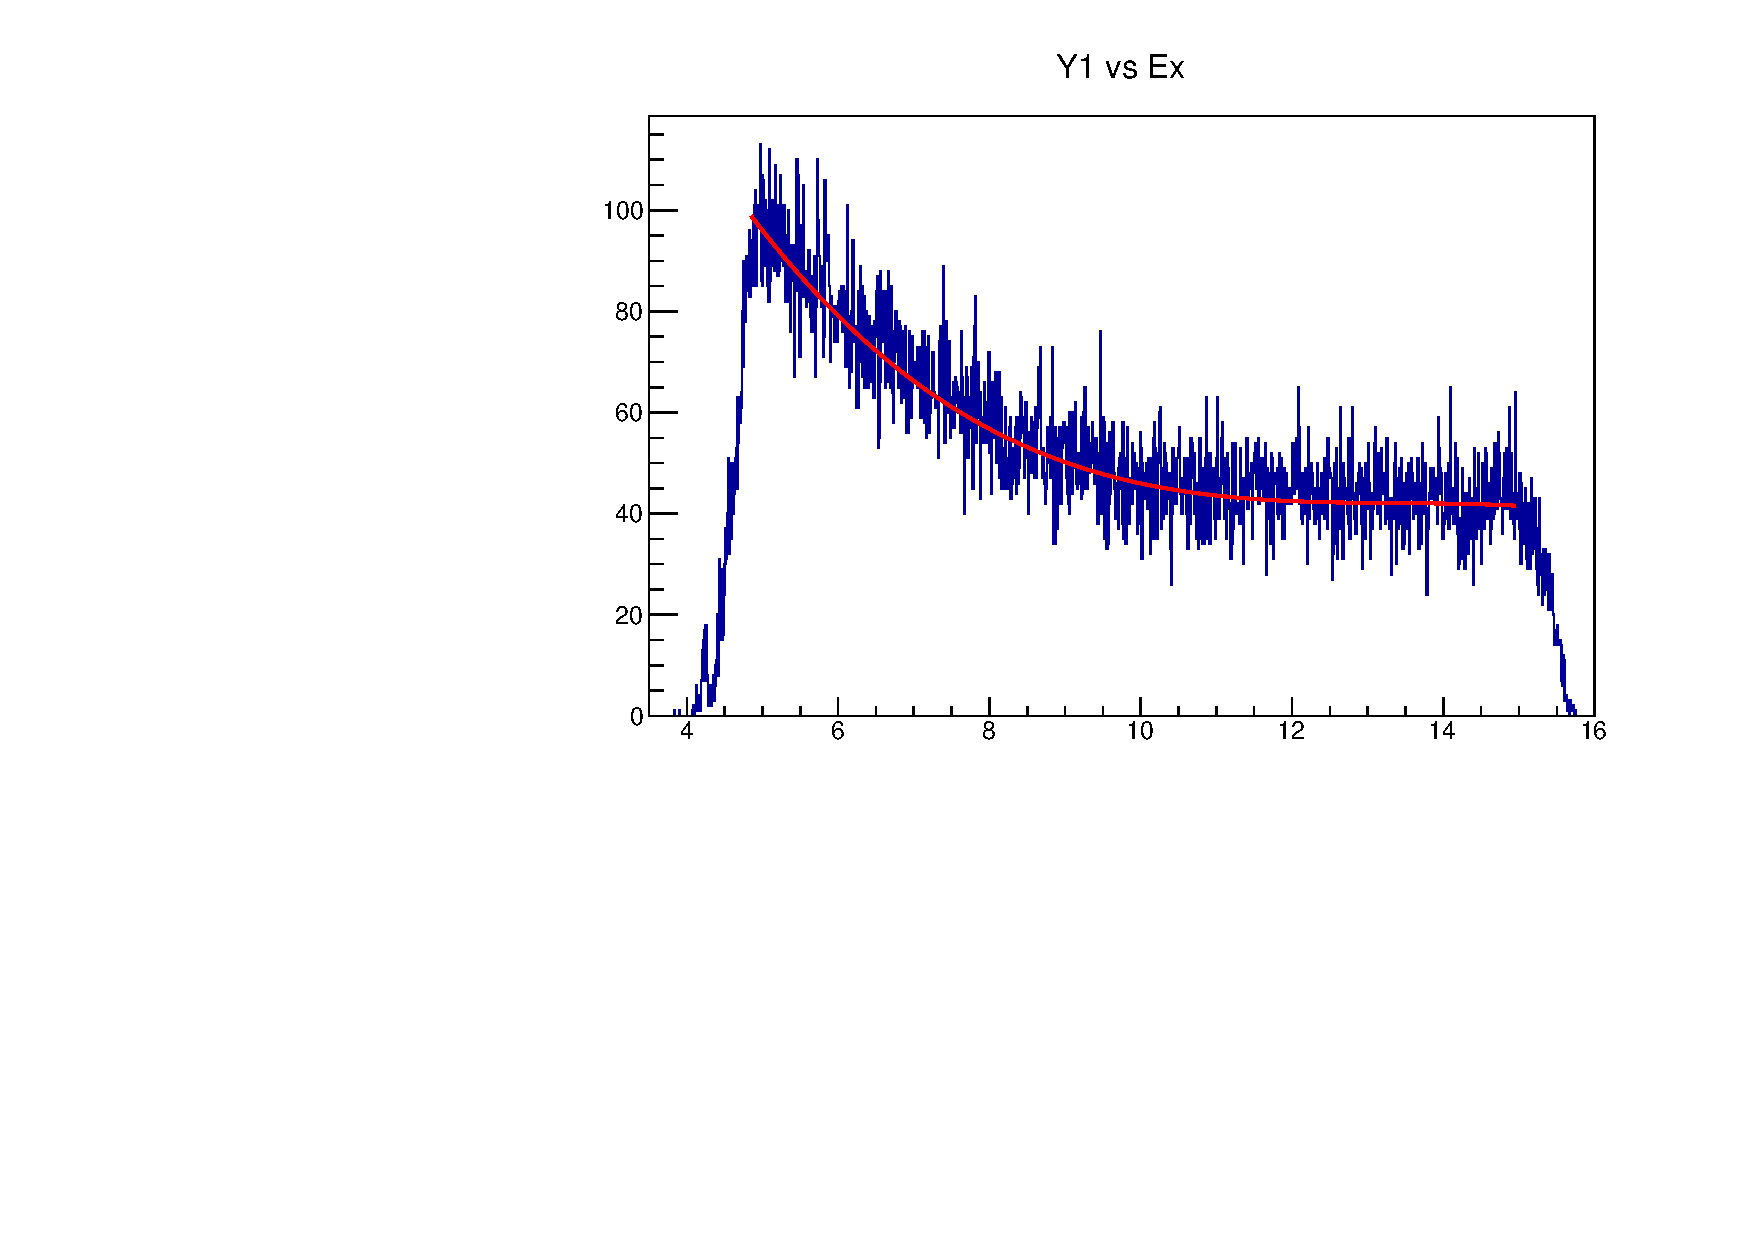
\includegraphics[width=\linewidth]{Figure/bkg/Chained_24Mg_bkg_projection_35_25.pdf}
			\caption{Ex projection of the background define by the dashed black lines in Fig. \ref{fig:Y1vsEx_orizline}.}
			\label{fig:Ex_bkg}
		\end{figure}

		\begin{figure}
			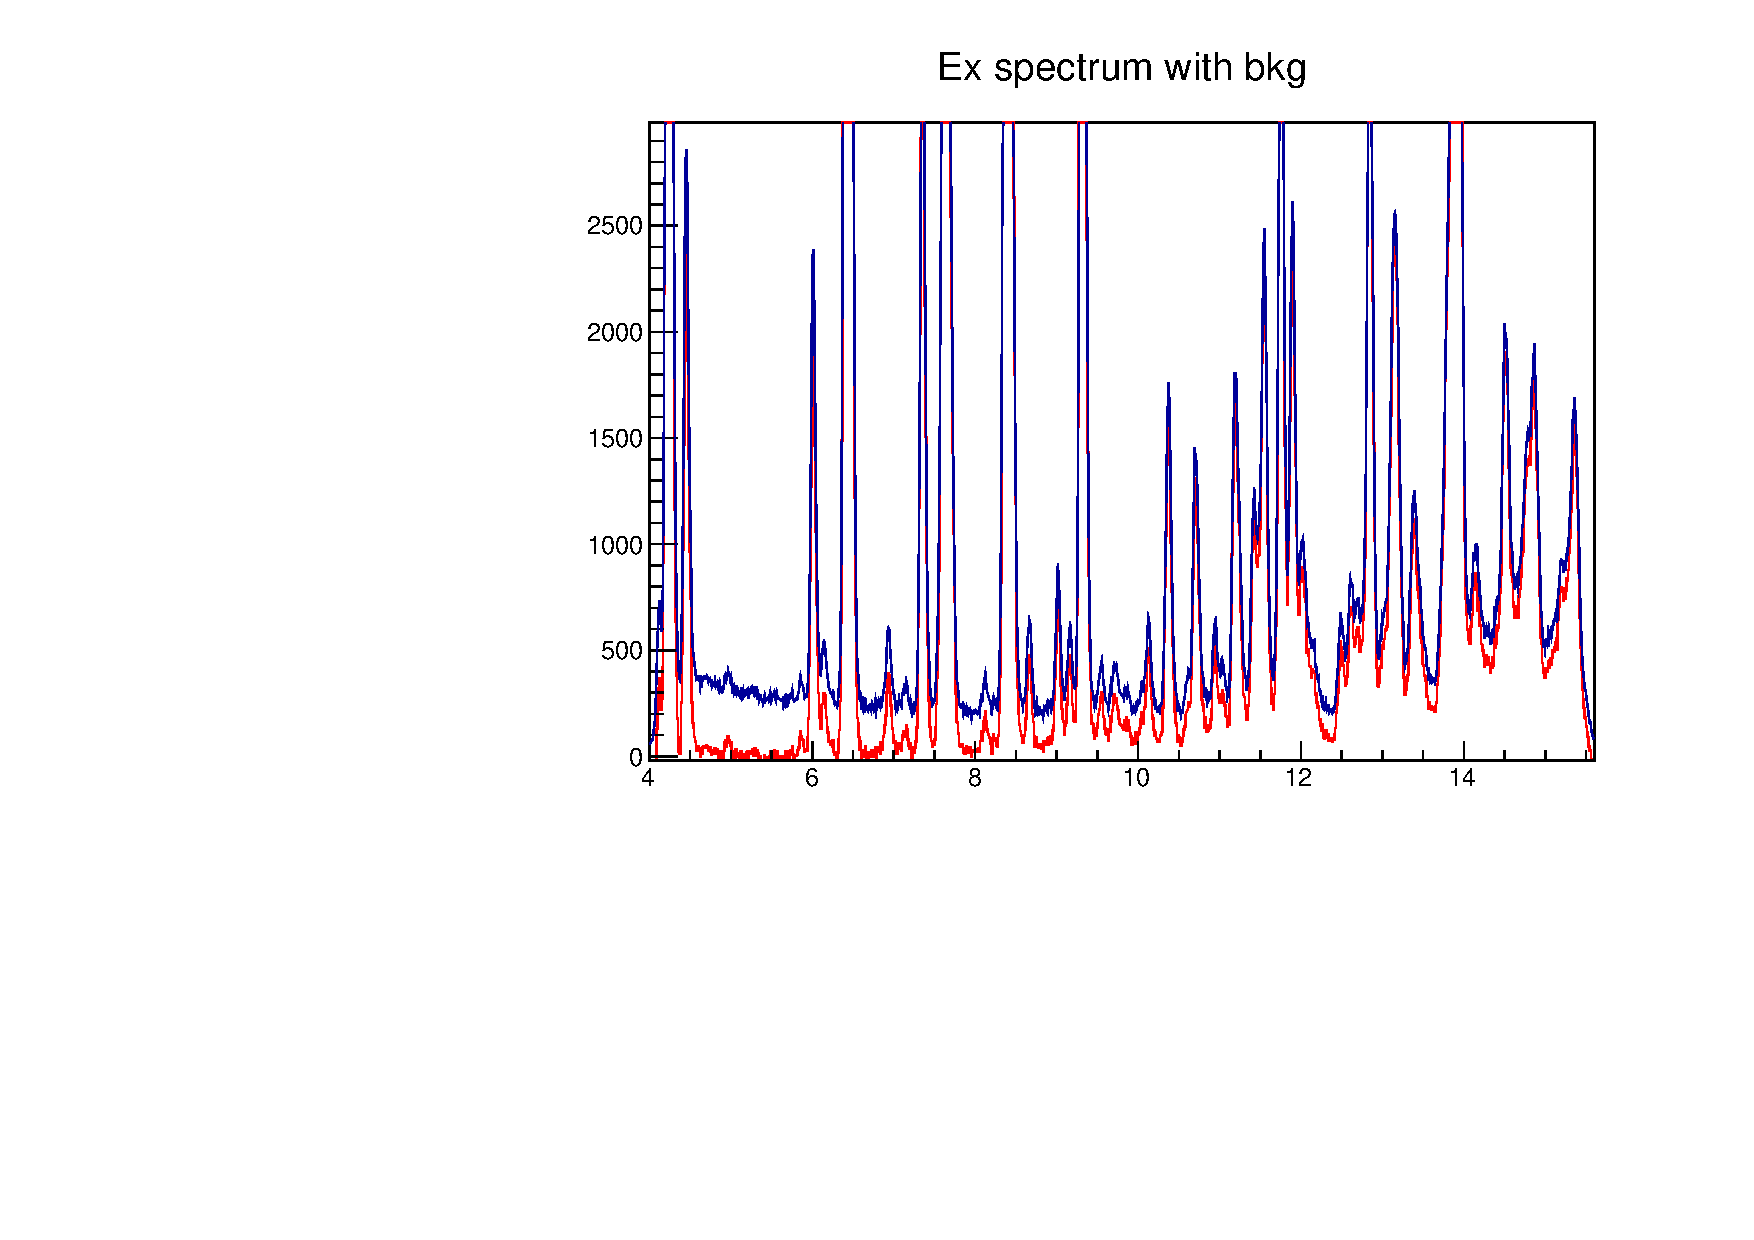
\includegraphics[width=\linewidth]{Figure/bkg/Chained_24Mg_Ex__withandwithout_bkg.pdf}
			\caption{Ex spectrum for 24Mg target. In red the background subtracted spectrum is shown.}
			\label{fig:Ex_bkgandnobkg}
		\end{figure}



\chapter{BaGeL Calibration}
\section{LaBr$_3$:Ce}





\end{document}
